\chapter{La physique des neutrinos}
    \chapterprecishere{
        ``Potentielle citation sans aucun rapport avec le sujet"\par\raggedleft--- \textup{Personne inconnue}, contexte à déterminer
    }
    
    Le projet WA105/protoDU$\nu$E teste la technologie de détecteur \gls{lartpc} à l'échelle du kilotonne dans le but d'être utilisée dans la future expérience de physique des neutrinos \gls{dune}. Le but de ce chapitre est de montrer en quoi la physique des neutrinos est un domaine de la physique des particules offrant des possibilités de nouvelles découvertes, et comment la future expérience \gls{dune}, sera capable de s'y attaquer. Dans un premier temps, la place du neutrino dans le modèle standard de la physique des particules est présentée par une approche historique. Dans un second temps, le phénomène de l'oscillation des neutrinos est décrit afin d'expliquer comment l'expérience \gls{dune} pourra s'attaquer à des questions comme l'asymétrie matière-antimatière dans l'univers.
    
    \section{De la nécessité théorique à la place du neutrino dans la modèle standard}
    
	    \subsection{Brève histoire de la physique des particules}
	    
		    \begin{figure}[htpb!]
		    	\centering
		    	\includegraphics[width=0.8\textwidth]{SM.png}\\
		    	\tiny{By L. Boyle, modified by P. Cotte. Creative Commons SA}
		    	\caption[Le modèle standard de la physique des particules.]{\label{fig::SM}Le modèle standard de la physique des particules. Voir encadré \ref{box::SM}.}
		    \end{figure}
		    \begin{figure*}[htpb!]
			    \begin{activitybox}[label=box::SM]{Le modèle standard de la physique des particules}
			    	La \autoref{fig::SM} schématise le modèle standard de la physique des particules tel que nous le comprenons aujourd’hui. Il repose sur un concept de symétrie et de brisure de symétrie. La ligne du haut représente l'univers dans ses premiers instants ($\sim\SI{e-11}{\second}$), avant que la température moyenne ne descende en dessous du seuil de \SI{160}{\giga\electronvolt}. Le potentiel de Higgs $V(H)$ (colonne de droite) était alors symétrique, et son minimum correspondait à un champ de Higgs $H$ nul. Toutes les particules étaient alors de masse nulle. La seconde ligne décrit l'univers tel qu'il est aujourd'hui. Quand la température de l'univers est passé en dessous de \SI{160}{\giga\electronvolt}, le minimum du potentiel de Higgs correspondait à un champ non nul, baignant tout l'espace et avec lequel les particules interagissent pour acquérir leur masse.
			    	
			    	Les deux tableaux du milieu décrivent les fermions, les particules de spin demi-entier. Ils constituent ce qui est communément appelé "matière", contrairement aux bosons de la dernière colonnes qui sont les médiateurs des interactions et ne sont donc pas de la matière. Il existe deux versions de chacune de ces particules : une de chiralité gauche, portant un isospin faible demi-entier sensible a l'interaction faible, et une de chiralité droite avec un isospin faible nul, insensible à l'interaction faible. Les deux premières lignes correspondent aux quarks ($u$, $d$, $c$, $s$, $t$ et $b$), particules de charge électrique non-entière et portant une charge de couleur, leur permettant de former la matière hadronique via l'interaction forte et ne pouvant exister seuls. Les deux dernières lignes correspondent aux leptons, insensibles à l'interaction forte. Les neutrinos  ($\nu_e$, $\nu_{\mu}$ et $\nu_{\tau}$) sont électriquement neutre et de masse très faible comparé aux autres particules. Ils peuvent se transformer en/être créés avec leur lepton associé (électron $e$, muon $\mu$ et tau $\tau$) en interagissant avec un boson $W^{\pm}$. Ces leptons portent une charge électrique élémentaire négative. La première génération (i.e colonne) de fermions, composée des quark up ($u$) et down ($d$), de l'électron et du neutrino électronique, correspond à la matière stable, celle qui constitue tout ce qui nous entoure. Les particules des deux autres générations sont instables (sauf les neutrinos) à cause de leur masse plus importante. Chaque fermion a un antifermion associé (qui ensemble forment l'antimatière), dont toutes les charges sont inversée mais qui a la même masse que le fermion.
			    	
			    	Les bosons quand à eux sont des particules de spin 1. Au nombre de 12, ils sont les médiateurs des interactions fondamentales. Les 8 gluons ($g$) se couplent par interaction forte à toutes les particules pourtant une charge de couleur. Ils portent chacun une charge et une anticharge de couleur, mais pas de charge électrique ni d'isospin faible. Les bosons massifs chargés $W^{\pm}$ et le boson massif neutre $Z^0$ sont médiateurs de l'interaction faible et se couplent à toutes les particules portant un isospin faible demi-entier (qu'il n'ont pas eux même). Le boson non massif neutre $\gamma$ (le photon) est médiateur de l'électromagnétisme et ne porte ni charge de couleur ni isospin faible. Ils sont tous les quatre des superpositions linéaires de bosons de masse nulle qui existaient avant la brisure de symétrie.
				\end{activitybox}
			\end{figure*}
	    
		    La physique des particules, dont le modèle standard est schématisé en \autoref{fig::SM}, est une discipline née de la convergence de l'électromagnétisme, de la mécanique quantique et de la relativité restreinte. Elle a pour objectif la compréhension du comportement des objets physiques à la plus petite échelle possible.
		    
		    La première pierre de la mécanique quantique est la discrétisation des rayonnements d'un corps incandescent suggéré par Max Planck en 1900\cite{Planck1900}, bien que ce dernier ne la voyait alors que comme un artifice mathématique correspondant bien aux observations. Einstein, en 1905\cite{Einstein1905-quanta}, se basera sur le travail de Planck et proposera la notion de quantum de lumière appelé plus tard "photon" pour expliquer les résultats expérimentaux de l'effet photoélectrique observés en 1839 par Antoine Becquerel et Alexandre Edmond\cite{Becquerel1839}. Il publie sa théorie de la relativité restreinte\cite{Einstein1905-relat}, qui permet de se passer de la notion d'éther luminifère, ainsi que la très célèbre équation $E=mc^2$\cite{Einstein1905-emc2} la même année. La mécanique quantique continuera à s'étoffer jusqu'en 1930 avec les travaux de Bohr, de Broglie, Pauli, Schrödinger et Heisenberg pour aboutir à l'interprétation de Copenhague\cite{Heisenberg1949}, qui constitue un nouveau paradigme où la notion de probabilité n'est plus juste issue d'un manque de connaissance mais est une propriété intrinsèque des systèmes. C'est à cette période que Pauli propose l'existence du neutrino\cite{Pauli1930}, nouvelle particule pas encore observée à ce moment là mais dont l'existence est nécessaire au maintien du principe de conservation de l'énergie (voir \autoref{sec::neutrino_origin}).
		    %RAJOUTER ENCADRE SUR U(1)? Ou faire une annexe?
		    Viennent ensuite les théories des interactions fondamentales et des champs de particules. La nécessité d'une interaction forte, responsable de la cohérence du noyau atomique, est entrevue après les résultats de l'expérience de Rutherford, démontrant l'existence du noyau. Les bosons, particules de spin entier, sont nommés d'après Satyendranath Bose, qui proposa leur existence en 1923 afin d'expliquer les découvertes de Planck sur les quanta de lumière\cite{Bose1924}. En 1926, Oskar Klein et Walter Gordon\cite{Klein1926,Gordon1926} créent l'équation portant leurs noms, capable de décrire le comportement de particules de spin 0 (un cas particulier de bosons dont fait parti le célèbre boson de Higgs). En 1928, Dirac propose son équation d'onde relativiste décrivant les particules de spin demi-entier, appelé fermions en l'honneur d'Enrico Fermi\cite{Dirac1928}. Se faisant, il prédit au passage la possibilité de l'existence de l'antimatière, dont le premier représentant, le positron, sera découvert en 1933 par Carl D. Anderson\cite{Anderson1933}. Fermi propose sa théorie de l'interaction faible, expliquant la désintégration $\beta$ en 1934\cite{Fermi1934}, qui s'avérera être une approximation du modèle de Yukawa de 1935\cite{Yukawa1935} où les interaction se font via un échange de boson. Feynman, Schwinger et Tomonaga\cite{Tomonaga1946,Schwinger1948,Feynman1998} créent la théorie de l'électrodynamique quantique entre 1946 et 1950, première forme du modèle standard que nous connaissons aujourd’hui. Cette théorie promeut une propriété des équations de Maxwell au rang de principe : le fait que les équations de Maxwell soient apparemment invariantes sous certaines transformations des champs électriques et magnétiques. Cette invariance se traduit en mécanique quantique par l'invariance de la probabilité de présence d'une particule chargée sous un rephasage $U(1)$ pouvant dépendre de l'espace (transformation dite \textit{locale}). Imposer l'invariance sous cette transformation $U(1)$ locale du lagrangien libre de cette même particule chargée aboutit naturellement à l'apparition de termes d'interaction avec un champ de boson, qui n'est autre que le photon, médiateur de l'interaction électromagnétique. Une très bonne introduction à ce concept peut se trouver dans "Geometry, particles and fields", de Bjorn Felsager \cite{felsager}.
		    
		    S'en suivent alors les découvertes de très nombreuses particules : de nombreux mésons, baryons et  hadrons, ainsi que le lepton $\mu$, ou muon, qui avait été découvert en 1937\cite{Street1937}. Les théories de Yang et Mills de 1954\cite{Yang1954} généralisent l'invariance de jauge $U(1)$ de l'électrodynamique quantique et seront utilisées par Gell-Mann en 1961-1964\cite{Glashow1961,Gell-Mann1964} pour créer la chromodynamique quantique, qui décrit l'interaction forte responsable de la cohésion du noyau atomique, en imposant au lagrangien une invariance par transformation $SU(3)$. La notion de quarks, composants fondamentaux du zoo de particules alors connues, est pensée par la même occasion. Glashow, Salam et Weinberg imposent une invariance $U(1)\otimes SU(2)$ en 1967\cite{Glashow1961a,Salam1964,Weinberg1967} pour unifier les interactions faible et électromagnétique, et la brise en utilisant le mécanisme de brisure de symétrie postulée en 1964 par  Brout, Englert, Higgs, Hagen, Guralnik et Kibble\cite{Englert1964,Higgs1964,Higgs1964a,Kibble1967} prédisant l'existence du fameux boson de Higgs pour expliquer la génération des masses des particules massives alors connues. 
		    
		    Le neutrino électronique est découvert en 1956 par Cowan et Reine\cite{Cowan1956} auprès d'un réacteur nucléaire et le neutrino muonique est observé en 1962\cite{Danby1962} au synchrotron AGS à Brookhaven. 30 ans séparent la proposition de l'existence du neutrino par Pauli et sa découverte. Le lepton $\tau$ est découvert en 1976\cite{Perl1975} avec l'anneau de collision SPEAR à SLAC, les bosons $Z^0$ et $W^{\pm}$, médiateurs de l'interaction faible, en 1983\cite{Arnison1983,Arnison1983a} avec l'expérience UA1 du CERN. Le dernier quark, le top, est découvert en 1995\cite{Collaboration1995} au Fermilab. Le neutrino tauique est découvert en 2000 par l'expérience DONUT\cite{Collaboration2000} au Fermilab également et finalement le boson de Higgs est découvert en 2012 au LHC du \gls{cern}\cite{Collaboration2012}. Toutes les particules prédites et décrites par le modèle standard de la physiques des particules, dont une représentation est montrée en \autoref{fig::SM}, ont alors été observées. 
		    
		    Le puzzle du modèle standard est alors complet, et seul quelques phénomènes rares restent encore à observer. Tout ceci laisse cependant les physiciens sur leur faim : le modèle standard ne prédit pas tout (matière noire, gravitation...) et présente des particularités qui semblent être des manifestations de phénomènes sous-jacents, notamment les grandes différences entre les masses des trois générations de particules (les trois colonnes "fermions" de la \autoref{fig::SM}). En d'autres endroits, le modèle standard semble même en désaccord avec les observations, par exemple concernant le moment magnétique du muon, où un désaccord entre la théorie et l'expérience de \numprint{3.5}$\sigma$ est observée\cite{pdg2018}. Des théories au-delà du modèle standard sont alors mises au point, comme la supersymétrie ou la théorie des cordes\cite{pdg2018}. Mais cette quête de nouvelle physique est pour le moment peu concluante : aucune particule supersymétrique n'a été détectée et les énergies actuelles ne permettent pas de tester bon nombre de nouvelles théories.
		    
		    L'avenir de la physique des particules été alors un peu sombre, jusqu'aux observations à la fin du XX$^{\text{ème}}$ et au début du XXI$^{\text{ème}}$ siècle du phénomène d'oscillation des neutrinos par les expériences Super-Kamiokande\cite{Fukuda1998} et SNO\cite{Aharmim2013}. Ces particules avaient joué un rôle secondaire dans le modèle standard jusque là. Le neutrino était certes nécessaire au maintien du principe de conservation de l'énergie, mais il avait peu de pouvoir prédictif. Il avait cette particularité d'être de masse nulle, et de se coupler uniquement à l'interaction faible, contrairement aux autres particules : les leptons (électron, muon et tau) se couplent aussi à l'électromagnétisme, et les quarks se couplent aux trois interactions\footnote{Toutes ces particules peuvent également se coupler à la gravitation, mais cette interaction n'est pas décrite par le modèle standard.}. Mais Super-Kamiokande et SNO ont observé qu'un neutrino initialement produit par un électron, donc dans un état de saveur électronique, peut produire à sa détection un neutrino d'une autre saveur, muonique ou tauique. Cette capacité qu'ont les neutrinos à changer de saveur est ce que l'on appelle "oscillation des neutrinos" et, comme nous allons le voir plus loin, elle requiert que les neutrinos aient une masse non nulle. Ce qui n'est pas prédit par le modèle standard de la physique des particules, et donc constitue de la nouvelle physique.
		    
		    Avant de rentrer dans les détails des oscillations des neutrinos, nous allons présenter un peu plus les caractéristiques de la particule la plus discrète du modèle standard.
		    		    
    
        \subsection{Le spectre d'énergie des électrons de désintégration \texorpdfstring{$\beta$}{b} : besoin d'une nouvelle particule}\label{sec::neutrino_origin}
        
	        \begin{wrapfigure}{R}{0.5\textwidth}
	        	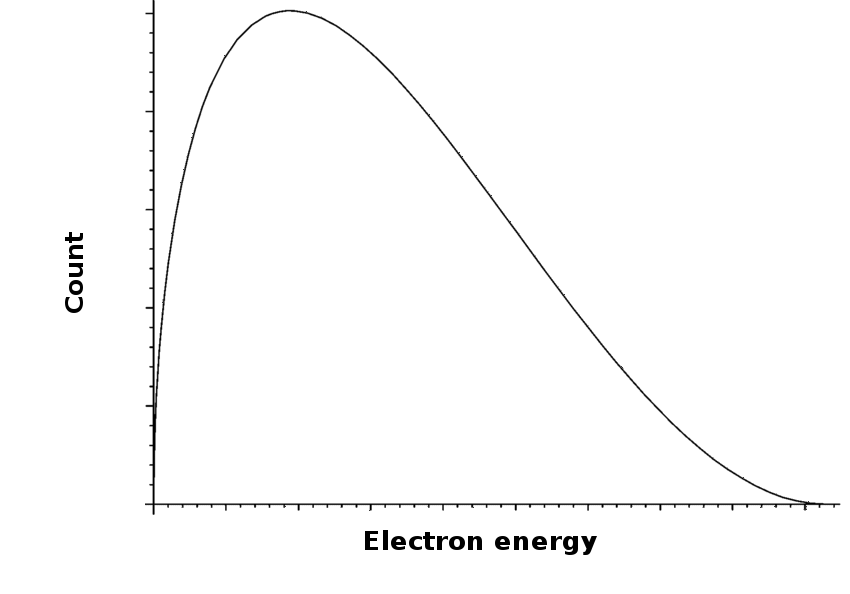
\includegraphics[width=0.5\textwidth,keepaspectratio]{beta_spectrum.png}
	        	\caption[Spectre de désintégration $\beta$.]{\label{fig::beta_spectrum}Spectre de l'énergie d'un électron émis par une désintégration $\beta$ d'énergie $Q$. Le fait qu'il soit continue entre 0 et $Q$ indique qu'une autre particule est émise en même temps que l'électron.}
	        \end{wrapfigure}
	        La désintégration $\beta$ est la transformation spontanée d'un neutron d'un noyau atomique en proton via l'émission d'un électron et d'un antineutrino électronique. L'énergie émise par une telle désintégration est égale, d'après la formule d'Einstein, à la différence des masses des noyaux avant et après désintégration multipliée par la vitesse de la lumière au carré : 
	        \begin{equation}
	        	Q = \left[m\left(^A_Z X\right)-m\left(^A_{Z+1} X\right)\right]c^2
	        \end{equation}
	        Pour un type de noyau $\left(^A_Z X\right)$, cette énergie est constante. La conservation de l'énergie nous dit alors que
	        \begin{equation}
	        	E_{initial} = E_{final} +E_{e^-}+E_{\overline{\nu}_e} = E_{final}+Q
	        \end{equation}
	        où $E_{initial}$ est l'énergie totale du noyau avant désintégration, $E_{final}$ est son énergie après désintégration et $E_{e^-}$ et $E_{\overline{\nu}_e}$ sont les énergies de l'électron et de l'antineutrino. On a donc $E_{e^-}+E_{\overline{\nu}_e} = Q$.
	        
	         Au moment de la proposition de l'existence du neutrino par Wolfgang Pauli en 1930\cite{Pauli1930}, seul l'électron et le noyau après désintégration étaient détectables, aussi le terme d'énergie $E_{\overline{\nu}_e}$ était absent de l'équation précédente. Dans ce cas, pour une source radioactive donnée, puisque $Q$ est constante, le spectre en énergie de l'électron aurait due être très piqué atour de $Q$. Or ce n'est pas le cas : ce spectre est continue (voir \autoref{fig::beta_spectrum}) entre 0 et $Q$. En revanche, rajouter à la réaction une particule jusque-là invisible correspond parfaitement à ce spectre, pourvu que la masse de cette particule soit très petite devant $Q$. En effet, si l'antineutrino (et donc le neutrino) avait une masse conséquente, le spectre de l'énergie de l'électron ne pourrait pas atteindre la valeur de $Q$, puisqu'un partie irréductible de $Q$ irait dans la masse du neutrino. C'est d'ailleurs un mesurant avec une très grande précision le spectre de l'énergie des électrons issues de la désintégration du tritium que l'expérience KATRIN\cite{Kleesiek2018} vise à déterminer la masse effective du neutrino électronique avec une précision de \SI{0.2}{\electronvolt\per c\squared}.
    
        \subsection{Premières observations directes du neutrino}
        
	        Entre les années 30 et 50, la détection du neutrino semblait hors de portée. Il était connu que la probabilité d'interaction de cette particule étant très faible, seule un source très intense de neutrinos pouvait permettre leur observation. Le développement de l'énergie nucléaire dans les années 50 a fourni cette source : les réactions de fission sont accompagnées de l'émission d'antineutrinos électroniques en très grande quantité.
	        
	        Entre 1952 et 1953, Frederick Reines et Clyde Cowan construisent un détecteur dont le matériau de réaction est simplement de l'eau. Un antineutrino incident, quand rencontre un proton, fait une réaction $\beta$ inverse produisant un neutron et un positron, se dernier s'annihilant rapidement avec un électron pour donner deux photons. Le signal attendu est alors la détection de deux photons suivie par l'interaction d'un neutron avec l'eau caractérisée par l'émission d'un troisième photon, après absorption du neutron par un noyau de chlorure de cadmium, un bon absorbeur de neutron que Reines et Cowan avaient dissous dans l'eau. La détection des photons s'effectuaient dans une couche de scintillateur liquide munie de tubes photomultiplicateurs entourant les deux cuves de détection. Le volume d'eau total était de $\SI{200}{\liter}$ où étaient dissous $\SI{40}{\kilogram}$ de chlorure de cadmium. Le flux de d'antineutrinos attendu du réacteur était de l'ordre de $\SI{e13}{\overline{\nu}_e\second^{-1}\centi\meter^{-2}}$.
	    
		    La première tentative de détection du neutrino fut faite proche du réacteur nucléaire de Hanford dans l'état de Washington, sans donner de résultat concluant. La seconde tentative, proche du réacteur de Savannah River en Caroline du Sud, détecta un signal de \SI{2.88}{\text{coups}\per\hour}\cite{Cowan1956} pour 1371 heures de prises de données, 20 fois supérieur au bruit de fond attendu, démontrant finalement l'existence d'une particule légère, et particulièrement peu réactive, dans la réaction $\beta$. La section efficace mesurée de  \SI{6.3e-44}{\centi\meter\squared} était compatible avec la valeur tirée des mesures de désintégration du neutron de Robson\cite{Robson1951}, de \SI{6e-44}{\centi\meter\squared}.
		    
		    Aujourd'hui, les expériences cherchant à détecter des neutrinos sont conçues de manière semblable à l'expérience de Reines et Cowan : un volume aussi grand et aussi dense que possible afin d'offrir un maximum de protons cibles sur lesquels les neutrinos  peuvent interagir, une source de neutrinos intense et un temps d'exposition long. La réduction du bruit de fond est essentielle dans une telle expérience : lors de leur seconde tentative, Reines et Cowan ont en effet placé leur détecteur sous terre. Ceci leur a permit de réduire grandement le taux de rayons cosmiques arrivant dans leur détecteur. En effet, ces derniers étaient susceptibles de créer des signaux semblables à celui attendu pour une interaction neutrino. Cette technique est encore largement employée aujourd'hui dans les expériences détectant des neutrinos.
		    
		    L'eau est encore utilisée aujourd'hui pour détecter des neutrinos, par exemple dans l'expérience Super-Kamiokande\cite{Fukuda1998}, mais des détecteurs solides ont également vu le jour comme dans les expériences NO$\nu$A\cite{Adamson2016} et OPERA\cite{Agafonova2018}. Une des techniques les plus récentes utilise comme cible des gaz nobles liquéfiés, plus dense que l'eau, notamment l'argon dans l'expérience prototype ICARUS\cite{Amerio2004} et la future expérience \gls{dune}\cite{Acciarri2016a}. 
		    
		    Les réacteurs nucléaires sont encore beaucoup utilisés dans les expériences de neutrinos, par exemple par Double Chooz\cite{Crespo-Anadon2014}, Daya Bay\cite{An2014}, RENO\cite{Collaboration2010} et la future JUNO\cite{An2015}. Les faisceaux de neutrinos créés artificiellement, plus contrôlables que les réacteurs, ont été inventés dans les années 60. L'expérience T2K\cite{Abe2018} détecte des neutrino issus d'un faisceau, et ce sera le cas également de l'expérience \gls{dune}\cite{Strait2016}. Des sources naturelles existent aussi : le soleil fourni un important flux de neutrinos, étudiés par des expériences comme SNO\cite{Aharmim2013}. Cette dernière, avec Super-Kamiokande\cite{Fukuda1998} qui détecte des neutrinos produits par des rayons cosmiques dans l'atmosphère, a permis de mettre en évidence le phénomène d'oscillation des neutrinos dont nous parlerons en détail dans la prochaine section. Les deux expériences ont reçu le prix Nobel de physique en 2015. Enfin, les neutrinos issus de supernovae peuvent également être détectés, pourvu qu'une supernovae explose durant une prise de données d'une expérience. C'est arrivé une seule fois en 1987, où 20 événements neutrinos ont été détectés par les détecteur IMB et Kamikande II\cite{Hirata1987}.

		\subsection{Les 3 familles de neutrinos}
		
			\begin{wrapfigure}{R}{0.5\textwidth}
				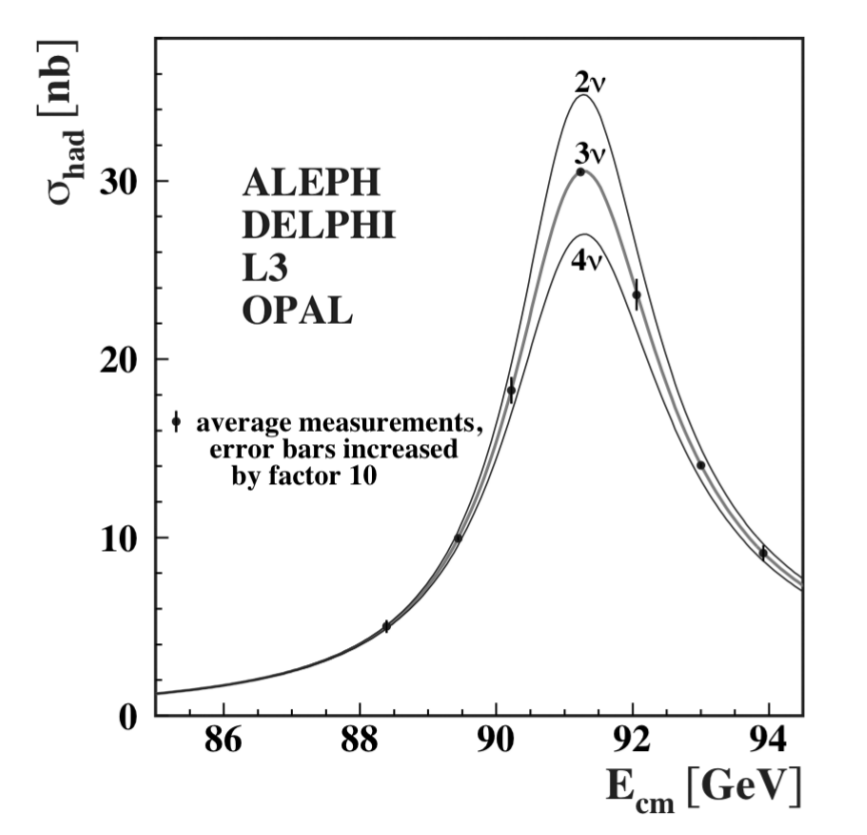
\includegraphics[width=0.5\textwidth,keepaspectratio]{three_neutrinos.png}
				\caption[Spectre de désintégration $\beta$.]{\label{fig::three_neutrinos}Mesure de la section efficace de production de hadron en fonction de l'énergie dans le centre de masse au LEP autour de la masse du boson $Z^0$. Résultats combinés des quatre expériences. Les courbes représentent les prédictions théoriques pour un nombre de saveurs de neutrinos actifs de 2, 3 et 4, les points sont les résultats de mesures, qui montre qu'il y a 3 familles de neutrinos actifs. Les incertitudes sont agrandies d'un facteur 10. Graphique tiré de \cite{Mele2015}.}
			\end{wrapfigure}
			Le muon, découvert en 1937 par Street et Stevenson\cite{Street1937}, n'a a priori comme différence avec l'électron que sa masse. Ce dernier étant (théoriquement, à l'époque) produit avec un neutrino dans les désintégrations $\beta$, il paraissait plausible que le muon puisse également être lié au neutrino d'une manière ou d'une autre.  Le spectre en énergie de l'électron produit par la désintégration du muon, mesuré par Leighton, Anderson et Seriff en 1949\cite{Leighton1949}, est continu. Un raisonnement identique à celui de Pauli de 1930 montre que le muon doit se désintégrer en trois particules : un électron et deux neutrinos. Il fallut cependant attendre 1962 et les expériences sur faisceau de neutrinos de Lederman, Steinberger et Schwartz\cite{Danby1962} pour détecter le neutrino muonique et définitivement montrer qu'il était différent du neutrino électronique : les neutrinos du faisceau, produits par la désintégration de muons, ne créaient que des muons dans le détecteur et aucun électron\footnote{Proche de la source, la probabilité  de changement de saveur lié au phénomène des oscillations des neutrinos est trop faible pour induire une composante autre que du neutrino muonique.}.
			
			La découverte du troisième lepton, le $\tau$, en 1975 par Perl\cite{Perl1975} n'a pas tardé à être suivi par la prédiction d'un troisième neutrino associé, le neutrino tauique. Ce dernier fut détecté en 2000 par l'expérience DONUT\cite{Collaboration2000}. Un faisceau de neutrinos issu du Fermilab, contenant toutes les saveurs possibles de neutrino, interagit avec un détecteur capable d'identifier les produits de réactions. Ce dernier a observé 4 événements neutrinos ayant créé un $\tau$.
			
			Les trois familles de quarks up--down, strange--charmed et top--bottom et les trois familles de leptons, l'électron et son neutrino, le muon et son neutrino et le tau et son neutrino, avaient alors été observées. Les quatre expériences du LEP, en étudiant la production de hadron à une énergie dans le centre de masse autour de la masse du boson $Z^0$, un des vecteurs de l'interaction faible, avait montré en 1989 qu'il ne pouvait pas exister plus de 3 saveurs de neutrinos sensibles à l'interaction faible\cite{DeCamp1989} (un graphique de cette étude est présenté en \autoref{fig::three_neutrinos}). Tous les neutrinos que nos instruments permettent de voir avaient alors été observés.
		    
		\subsection{Les symétries discrètes du modèle standard}\label{sec::CP}
		
			Un des principes fondamentaux du modèle standard, au même titre que la conservation de l'énergie, est que toute prédiction de ce dernier doit être identique après conjugaison Charge-Parité-Temps (CPT). Autrement dit, après avoir inversé la charge et les coordonnées spatio-temporelles.
			
			La conjugaison de charge inverse les charges -- électrique, isospin faible et couleur -- d'une particule. Un électron, par exemple, est transformé en positron, et de manière plus générale n'importe quelle particule chargée en son antiparticule. La transformation de parité consiste à prendre un système ou processus physique  et à le regarder dans un miroir. Autrement dit, remplacer toutes les coordonnées d'espace par leur opposées : $\Vec{r}\to-\Vec{r}$. Si la parité laisse le système ou processus inchangé, ce dernier est dit pair. Si au contraire il devient son opposé, il est dit impair. Un bon exemple de grandeur impaire est l'impulsion : $\Vec{p}(-\Vec{r}) = m(-\dot{\Vec{r}}) = -\Vec{p}(\Vec{r})$. À l'inverse, une grandeur paire est le moment cinétique : $\Vec{L}(-\Vec{r}) = -\Vec{r}\times -\Vec{p} = \Vec{L}(\Vec{r})$. L'extension à la mécanique quantique consiste à dire qu'un état est pair(impair) si il est état propre de l'opérateur de conjugaison de parité $\hat{P}$, qui inverse les coordonnées d'espace, avec une valeur propre de $+1(-1)$. Dans le modèle standard, une particule de spin $1/2$ est représentée par un spineur de Dirac $\psi(x,t)$, qui est composée de deux spineurs de Weyl :
			\begin{equation}
			\psi(x,t)=\left(\begin{matrix} u_R(x,t) \\ u_L(x,t)\end{matrix}\right)
			\end{equation}
			où $R$ et $L$ signifie "droite"(right) et "gauche"(left). Ils sont caractérisés par la manière dont un boost de Lorentz agit sur eux : ils acquièrent tous deux un facteur de phase, mais ces deux phases sont de signe opposé. Une transformation de parité transforme $u_R$ en $u_L$ et inversement. La dernière caractéristique importante d'un spineur de Weyl est qu'il est de masse nulle, alors qu'un spineur de Dirac peut avoir une masse $m_D$ : le lagrangien libre de Dirac, qui décrit comment évolue un spineur de Dirac sans interaction, autorise un terme de masse de la forme
			\begin{equation}\label{eq::dirac_mass}
			-m_D(\overline{u}_R u_L + \overline{u}_L u_R)
			\end{equation}
			où $\overline{u}_{R/L}$ est le conjugué de Dirac de $u_{R/L}$. Autrement dit, un fermion massif doit nécessairement avoir ses deux composantes gauche et droite non nulles. En revanche, il est possible qu'un fermion de masse nulle n'existe que dans un état de chiralité, gauche ou droite, auquel cas il peut être décrit par un spineur de Weyl $u_{R/L}$ seul. 
			
			La transformation de temps revient à inverser la flèche du temps et donc à regarder un processus dans l'autre sens. Par exemple, l'annihilation d'un électron avec un positron pour donner un photon devient l'émission d'une paire électron-positron par un photon.
			
			\begin{wrapfigure}{R}{0.5\textwidth}
				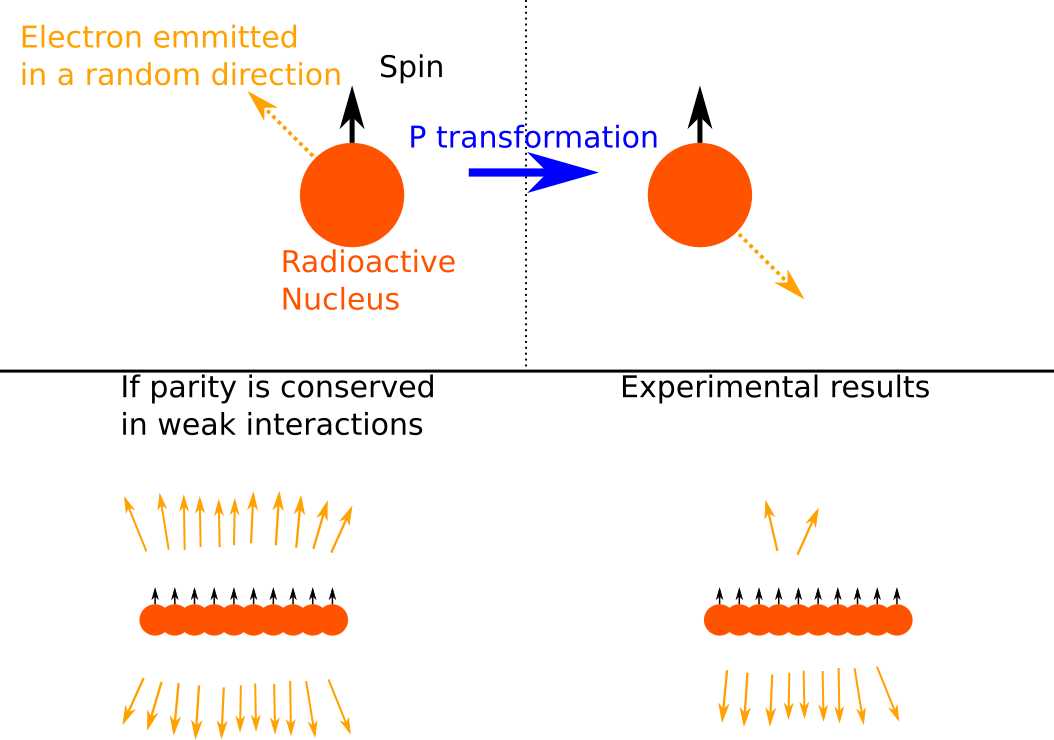
\includegraphics[width=0.5\textwidth,keepaspectratio]{wu2.png}
				\caption[Principe de l'expérience réalisée par C.S. Wu en 1957.]{\label{fig::wu}Principe de l'expérience réalisée par C.S. Wu en 1957 : un groupe de noyaux radioactif dont les spins sont tous orientés dans la même direction doivent émettre des électrons de manière isotrope si la conjugaison de partié est une symétrie de l'interaction faible. Il a été observer que les électrons étaient en majorité émis dans la direction opposée au spin, démontrant la violation de la symétrie $P$ par l'interaction faible.}
			\end{wrapfigure}
			Jusqu'en 1956, tous les processus physiques observés étaient invariants par transformation de parité, et cette dernière était considéré comme une symétrie de la nature. Mais cette même année, Tsung Dao Lee et Chen Ning Yang\cite{Lee1956} se rendent compte que, bien que bon nombre d'expériences montrent que les interactions forte et électromagnétique sont en effet symétriques par transformation de parité, aucune n'a étudié la question pour l'interaction faible. Ils proposent alors plusieurs méthodes expérimentales permettant de tester la conservation de la parité de l'interaction faible. L'une de ces expériences est réalisée entre 1956 et 1957 par Chieng-Shiung. Elle consiste à étudier la distribution spatiale des électrons émis par des noyaux radioactifs $\beta$ avec des spins alignés. La \autoref{fig::wu} schématise le signal recherché : le spin est invariant par transformation de parité alors que l'impulsion change de signe. L'image miroir d'un noyau émettant un électron dans la même direction que son spin est donc le même noyau émettant cet électron dans la direction opposée au spin. Le processus miroir est donc différent du processus initial et donc, pour que la désintégration $\beta$ soit symétrique par rapport à la transformation de parité, il faut qu'un ensemble de noyaux radioactifs dont les spins sont alignés émettent en moyenne autant d'électrons dans la direction de leur spin que dans la direction opposée. Or, l'expérience montre que ce n'est pas le cas : l'électron est en écrasante majorité émis dans la direction opposée au spin\cite{Wu1957}. L'interaction faible viole donc la symétrie $P$. Tsung Dao Lee et Chen Ning Yang reçoivent le prix Nobel en 1957 pour ces travaux.
			
			L'expérience de Wu, et plus tard celle de Goldhaber\cite{Goldhaber1958} en 1957, ont montré que l'interaction faible n'agit que sur la composante de chiralité gauche d'un spineur de Dirac, autrement dit la composante $\psi_L(x,t)=\left(\begin{matrix}0 \\ u_L(x,t)\end{matrix}\right)$. C'est pour cela qu'elle ne conserve pas la symétrie P. La masse du neutrino étant alors considérée comme nulle, il était naturel d'utiliser un spineur de Weyl de chiralité gauche pour décrire le neutrino, et un spineur de Weyl de chiralité droite pour décrire l'antineutrino.
			
			Si le neutrino est de charge nulle, une conjugaison de charge ne saurait le changer en son antineutrino. En effet, ce dernier n'existe que dans un état de chiralité droite, il faut donc également appliquer un transformation de parité. On peut donc se poser la question suivante : la transformation CP est-elle une symétrie du modèle standard? Si c'est le cas, les neutrinos et les antineutrinos doivent se comporter de la même manière. De manière générale, toute la matière décrite par le modèle standard se comporterait alors comme l'antimatière. Mais ceci soulève alors une question encore plus fondamentale : pourquoi n'y a-t-il plus d'antimatière dans l'univers? En effet, les théories actuelles du big bang\cite{Canetti2012} montrent qu' il devait y avoir autant de matière que d'antimatière à la création de l'univers. Matière et antimatière s'annihilent si elles se rencontrent, l'univers devrait être composé essentiellement de vide et de photons. Or ce n'est pas le cas : l'antimatière a disparu et la matière est restée. Le phénomène, appelé baryogenèse, responsable de cette asymétrie est encore mal connu, mais le fait que l'antimatière ne se comporte pas tout à fait comme la matière est nécessaire\cite{Sakharov1991}. Une telle asymétrie doit exister si la transformation CP n'est pas une symétrie de l'univers.
			
			Il a été expérimentalement prouvé que la symétrie CP n'est pas conservée dans le secteur des quark\cite{Collaboration2006,Charles2004,Kobayashi1973}: la matrice de mélange CKM contient une phase complexe introduisant un comportement légèrement différent entre les quarks et les antiquarks. Mais la violation de CP dans ce secteur n'est pas suffisante pour expliquer la baryogenèse\cite{Riotto1998}. En revanche, l'observation d'une violation de CP dans le secteur des leptons peut l'expliquer\cite{Davidson2008}. Comme nous le montrerons plus loin, le phénomène d'oscillation des neutrinos introduit également une phase complexe pouvant créer une différence de comportement entre matière et antimatière.
        
        \subsection{La masse du neutrino : Dirac ou Majorana}\label{sec::dirac_majorana}
        
	      \begin{activitybox}[label=box::mass_term]{Comment construire un terme de masse dans un lagrangien?}
	        	Le lagrangien du modèle standard est construit en utilisant le rasoir d'Ockham : on choisi en priorité les termes les plus simples qui respectent les lois de la physique. Un terme de masse doit donc respecter les critères suivants :
	        	\begin{itemize}
					\item[$\bullet$] Être invariant de Lorentz (i.e respecter la relativité restreinte).
					\item[$\bullet$] Avoir la dimension d'une énergie (le lagrangien est une énergie).
					\item[$\bullet$] Il doit faire intervenir la particule dont il est la masse.
					\item[$\bullet$] Il doit être réel, donc faire intervenir le champ et son conjugué complexe.
	        	\end{itemize}
	        	Le terme le plus simple respectant tous ces critères est, pour un fermion décrit par un champ $\psi$, de la forme $-m\bar{\psi}\psi$.
        	\end{activitybox}
	        
	        Nous avons vu dans la section précédente qu'un neutrino sans masse peut être décrit par un spineur de Weyl. Depuis la mise en évidence de la masse des neutrinos par le phénomène d'oscillation, il est clair que cette description est insuffisante, un spineur de Weyl ne pouvant pas avoir de terme de masse dans un lagrangien de Dirac. L'extension la plus simple consiste à considérer le neutrino comme un spineur de Dirac et de lui adjoindre le terme de masse \eqref{eq::dirac_mass} (voir l'encadré \ref{box::mass_term} pour une explication sur comment créer un terme de masse). Dans ce cas, le neutrino aura une composante de chiralité droite non nulle, qui n'interagit avec aucune interaction du modèle standard. Il peut interagir par gravitation, mais cette dernière est bien trop faible pour être détectable à l'échelle de la physique des particules. 
	        
	        Il existe une autre possibilité pour un terme de masse du neutrino: par son absence de charge, le neutrino peut également être décrit par un fermion de Majorana, dont le terme de masse est très différent de celui d'un fermion de Dirac. Un spineur de Majorana a la particularité qu'il est sa propre antiparticule. Dans le modèle standard, seul le neutrino peut être décrit par un spineur de Majorana. En effet, les autres fermions ont une charge électrique, ils ne peuvent donc pas être leur propre antiparticule qui doit être de charge opposée. Dans ce cas là, un nouvel état de chiralité droite n'est pas nécessaire, et donc aucun neutrino stérile n'est introduit (une discussion plus détaillée ce trouve ici\cite{Petcov2013}).
	        
	        Nous avons écrit en section précédente le terme de masse d'un spineur de Dirac. Pour un neutrino dans un état propre de l'hamiltonien $\nu_i=\nu_R+\nu_L$, nous avons donc : 
	        \begin{equation}
	        	-m_D\overline{\nu}_R \nu_L + \text{conjugué complexe}
	        \end{equation}
	        Ce terme de masse est créé, comme pour les autres fermions, par interaction du champ de neutrino avec le champ de Higgs après brisure de symétrie via un couplage de Yukawa. Il n'implique pas forcément de physique au-delà du modèle standard.
	        
	        Un terme de masse de Majorana quant à lui est de la forme
	        \begin{equation}\label{eq::majorana_mass}
	        -\frac{1}{2}m_M\overline{\nu}_L^T C \nu_L + \text{conjugué complexe}
	        \end{equation}
	        où $C$ est la matrice de conjugaison de charge. Comme l'explique B. Kayser dans \cite{Kayser2009}, un tel terme ne peut pas être créé par un couplage de Yukawa, mais par une interaction plus complexe avec le champ de Higgs qui n'est pas décrite par le modèle standard. Un terme de masse de Majorana pourrait expliquer la petitesse des masses des neutrinos par le mécanisme dit de see-saw , qui prédit l'existence de neutrinos ultra-lourds (\numprint{e9}--\SI{e15}{\giga\electronvolt}). Si la symétrie CP n'est pas conservée, ces derniers se seraient désintégrés à l'origine de l'univers en produisant un peu plus de matière que d'antimatière (voir l'article deB. Kayser\cite{Kayser2005}).
	        
	        Les différences de comportement entre neutrino de Dirac et de Majorana sont difficiles à observer. La plus recherchée en ce moment est la désintégration double-beta sans émission de neutrino, qui n'est possible que si le neutrino est sa propre antiparticule. Aucun résultat concluant n'a été observé à ce jour\cite{Dolinski2019}.
    
    \section{Le paradigme des oscillations des neutrinos}
    
        \subsection{Genèse de la théorie}
    
            On désigne habituellement un neutrino par sa saveur : neutrinos électronique ($\nu_e$), muonique ($\nu_{\mu}$) ou tauique ($\nu_{\tau}$). Quand un lepton chargé (électron muon ou tau) interagit avec un boson $W$, il se transforme en un neutrino de saveur définie (appelons-le $\nu_{\alpha}$), correspondant à celle du lepton chargé. De la même manière, un neutrino d'une saveur donnée (appelons-le $\nu_{\beta}$) se transforme en un lepton chargé de même saveur après interaction avec un boson $W$. Rien, à priori, n'oblige $\nu_{\alpha}$ à être de même saveur que $\nu_{\beta}$. Le premier à avoir soulevé ceci est Bruno Pontecorvo, même si il ne l'a pas fait en ces termes. En effet, au moment de la publication de ses deux premiers articles\cite{Pontecorvo:1957cp,Pontecorvo:1957qd} sur le sujet à la fin des années 60, seul le neutrino électronique avait été découvert. Pontecorvo parlait de possible transition entre neutrino et antineutrino du fait que le neutrino soit neutre, inspiré par les travaux de Gell-Mann et Païs\cite{Gell-Mann1955} sur la conversion du $\overline{K^0}$ en  $K^0$. Dans son article suivant en 1968\cite{Pontecorvo1968}, tout en gardant la possibilité de conversion des neutrinos vers les antineutrinos, il introduit la possibilité d'une conversion du neutrino électronique vers le neutrino muonique, découvert en 1962\cite{Danby1962}. Il prédira également deux résultats importants :
            \begin{itemize}
                \item[$\bullet$] Si les masses des neutrinos ne sont pas nulles et que la charge leptonique n'est pas conservée, les neutrinos peuvent changer de saveur.
                \item[$\bullet$] Dans ce cas, le flux de neutrino en provenance du soleil doit être environ 2 fois plus faible que le flux attendu sans changement de saveur.
            \end{itemize}
            La première prédiction implique de la physique au-delà du modèle standard, puisque ce dernier suppose que les masses des neutrinos sont nulles. La seconde prédiction fut vérifiée en 1970 par la Brookhaven Solar Neutrino Experiment\cite{Bahcall1976}, qui trouva un facteur de déficit compris entre 2 et 3. Il ne s'agissait alors pas encore d'une preuve, d'autres théories pouvant expliquer ce phénomène. Les auteurs de \cite{Bahcall1976} font d'ailleurs part de leur doutes quant à la précision des modèles solaires utilisés. Néanmoins, ce résultats était un indice qui a incité les chercheurs à creuser la question.
            
            Le changement de saveur $\nu_e\rightleftharpoons\nu_{\mu}$ avait été envisagé également entre 1962 et 1963 par deux groupes de physiciens, Katayama, Matumoto, Tanaka et Yamada\cite{Nakagawa1963} puis par Maki,  Nakagawa et  Sakata\cite{Maki1962}. Ces quatre derniers donneront leurs noms, avec Pontecorvo, à la célèbre matrice \gls{pmns} décrite plus loin, qui gouverne les transitions de saveur des neutrinos. Leur point de départ était différent de celui de Pontecorvo, puisqu'ils visaient à créer une théorie unifiant les leptons et les hadrons. Ils sont également arrivés à la conclusion qu'un changement de saveur des neutrinos implique que ces derniers doivent avoir des masses non nulles.
            
            En 2015, Arthur~B.~McDonald et Takaaki Kajita ont reçu le prix Nobel de physique "pour la découverte des oscillations des neutrinos, qui montre que les neutrinos ont une masse". Les deux expériences ayant fait cette découverte sont SNO\cite{Aharmim2013} et Super-Kamiokande\cite{Fukuda1998}.
            
            \begin{figure}[htbp]
                \begin{subfigure}[t]{0.56\textwidth}
                    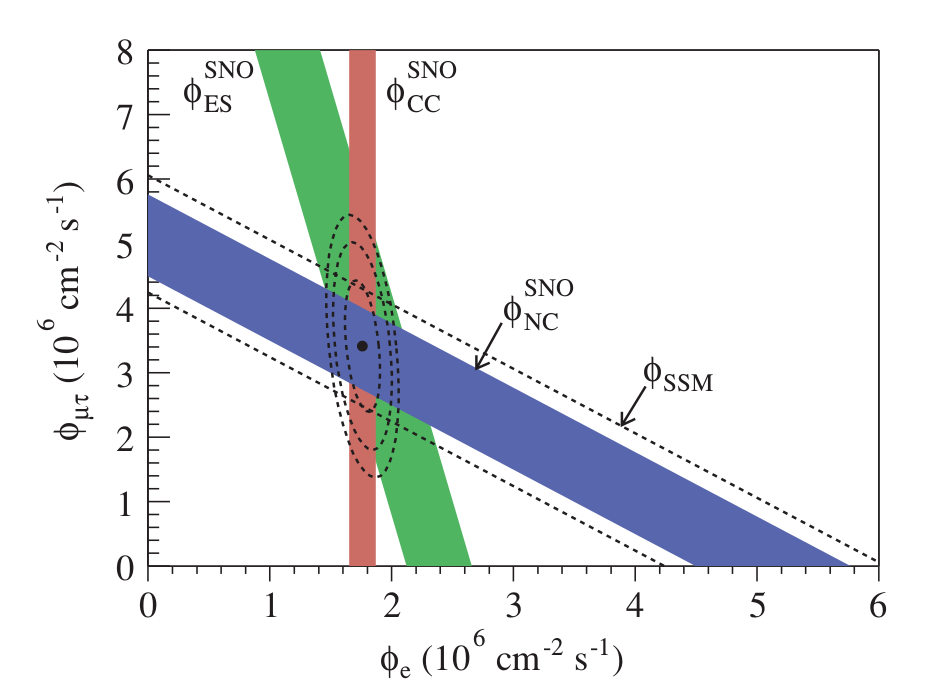
\includegraphics[width=\textwidth]{Chapitre_1/pictures/SNO_plot.png}
                    \caption{Composition $\nu_{\mu}$ et $\nu_{\tau}$ du flux des neutrinos solaires $^8$B en fonction de sa composition en $\nu_e$\cite{Aharmim2013}. La prédiction du modèle solaire est $\phi_{e}=\SI{5.15e6}{\nu\per\centi\meter\per\second}$. Les traits pointillés indiquent alors les valeurs possibles $\phi_{\mu\tau}$ et $\phi_e$ si les neutrinos peuvent changer de saveurs. Le flux mesuré par courant chargé $\phi_{CC}^{SNO}$ n'est sensible qu'aux $\nu_e$ et est donc égal à $\phi_{e}$. SNO l'a mesuré autour de $\SI{1.76e6}{\nu\per\centi\meter\per\second}$ (bande verticale rouge). Le flux mesuré par diffusion élastique $\phi_{ES}^{SNO}$ est égal à $\phi_{e}+0.1559\phi_{\mu\tau}$ (bande verte). SNO l'a mesuré autour de $\SI{2.39e6}{\nu\per\centi\meter\per\second}$. Le flux de courant neutre $\phi_{NC}^{SNO}$ est sensible de manière égale aux trois saveurs et est donc égal à $\phi_{e}+\phi_{\mu\tau}$, soit au flux total attendu. SNO le mesure autour de $\SI{5.09e6}{\nu\per\centi\meter\per\second}$, compatible avec la prédiction. Le fait que ces trois bandes s'interceptent en un même point indique que le flux total de neutrinos est en accord avec la prédiction, mais qu'il n'est pas composé uniquement de $\nu_e$, indiquant un changement de saveur.}
                    \label{fig::SNO_plot}
                \end{subfigure}
                \hfill 
                \begin{subfigure}[t]{0.4\textwidth}
                    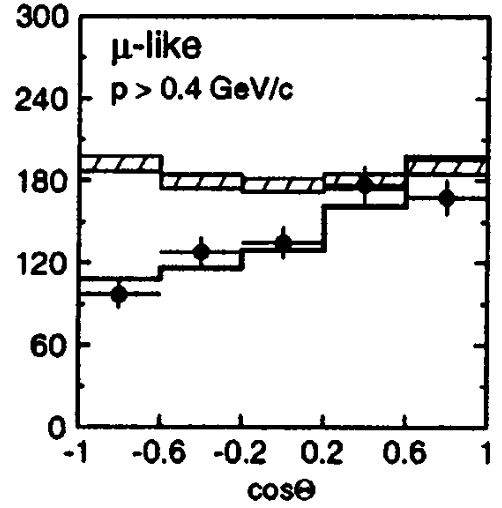
\includegraphics[width=\textwidth]{Chapitre_1/pictures/superK_plot.png}
                    \caption{Nombre de neutrinos muoniques mesurés par Super-Kamiokande (traits pleins) et prédit par le Monte Carlo en l'absence de changement de saveur (surfaces hachurées) pour un an et demi de prise de donnée, en fonction l'angle entre la verticale et la direction du neutrino\cite{Fukuda1998}. Un cosinus négatif correspond à un neutrino ayant traversé la Terre. La différence entre observation et prédiction à grand angle indique une disparition des neutrinos muonique à grande ligne de base.}
                    \label{fig::superK_plot}
                \end{subfigure}
                \caption[Les preuves que les neutrinos changent de saveur, par SNO et Super-Kamiokande.]{Les deux graphiques ayant prouvé les changement de saveur des neutrinos : le flux total de neutrinos provenant du soleil est conservé mais sa composition de saveur change, par SNO (gauche). Le nombre de neutrinos muoniques atmosphériques détectés dépend de la ligne de base, par Super-Kamiokander (droite).}
            \end{figure}
            
            SNO détectait les neutrinos solaires, par interaction par courant chargé (CC) et par courant neutre (CN), permettant d'avoir accès à la fois au flux de neutrinos électroniques (CN et CC) et au flux de neutrios muoniques et tauiques (CN). Comme le montre la \autoref{fig::SNO_plot}, la somme des trois flux correspond bien au flux total prédit par le modèle solaire standard alors que le flux de neutrinos électroniques est inférieur aux prédictions, montrant qu'une partie du flux change de saveur mais que le flux total est conservé.
            
            Super-Kamiokande détecte des neutrinos issus des interactions de rayons cosmiques avec l'atmosphère. Il pouvait ainsi comparer les flux des neutrinos pour différents angles zénithaux, correspondant à des créations du neutrino allant de juste au dessus du détecteur (angle nul) à l'autre bout du globe (angle de $\pi$). Comme nous allons le montrer plus loin, la probabilité qu'a un neutrino de changer de saveur dépend de la distance parcourue (équation \eqref{eq::proba_oscillation}). Une dépendance du flux en l'angle zénithal a donc indiqué un phénomène de changement de saveur dépendant de la distance. La \autoref{fig::superK_plot} montre cette dépendance pour des détections de neutrinos muoniques.
    
        \subsection{Pourquoi "Oscillations"?}\label{sec::oscillations}
            La base de la théorie des changements de saveur des neutrinos est de dire que les états $\nu_e$ $\nu_{\mu}$ et $\nu_{\tau}$ sont -- par définition -- des états propres du lagrangien d'interaction, mais pas forcément des états propres de l'hamiltonien, appelés également états propres de masse. Autrement dit, les états propres de saveur sont une composition linéaire des états propres de masse, et inversement. Il n'est donc pas possible de décrire la propagation dans l'espace-temps d'un état de saveur, bien que le neutrino soit créé et détruit dans un de ces états. Partant de là, nous allons montrer d'où provient le terme "oscillation".
            
            \subsubsection{Conventions de notation}
            \begin{itemize}
                \item[$\bullet$] $\hbar = c = 1$ (système d'unité naturelle)
                \item[$\bullet$] Nous supposerons que toutes les fonctions d'ondes décrites sont suffisamment loin de leur source pour être considérées comme des ondes planes. Les expériences de neutrinos vérifient généralement facilement cette condition.
                \item[$\bullet$] $\nu_e$, $\nu_{\mu}$ et $\nu_{\tau}$ sont les états propres de saveur. Un neutrino est dans un de ces états au moment de son interaction.
                \item[$\bullet$] $\nu_{\alpha,\beta...}$ désigne un des trois états propres de saveur.
                \item[$\bullet$] $l_{\alpha,\beta...}$ désigne un des trois leptons chargés $e$, $\mu$ ou $\tau$.
                \item[$\bullet$] $U_{\alpha i}$ est un élément de la matrice $U$ permettant de passer de la base des états propres de saveur à la base des états propres de masse.
                \item[$\bullet$] $\nu_{i}$ avec $i$ un entier non nul désigne un état propre de masse, qui vérifie l'équation
                \begin{equation}
                    \ket{\nu_i(t)} = e^{-i(E_i\cdot t - p_i\cdot x)}\ket{\nu_i(0)}.
                \end{equation}
                avec $E_i$ et $p_i$ l'énergie et l'impulsion du neutrino, constantes au cours du temps.
            \end{itemize}
            
            \subsubsection{Superposition des états de masse}
            Les états propres de saveurs, si ils ne sont pas des états de masses, sont une superposition linéaire de ces états. On peut donc écrire
            \begin{eqnarray}
            \ket{\nu_{\alpha}} = \sum_i U_{\alpha i}^*\ket{\nu_i} \label{eq::alphatoi} \\
            \ket{\nu_i} = \sum_{\alpha} U_{\alpha i}\ket{\nu_{\alpha}}.
            \end{eqnarray}
            L'état d'un neutrino initialement créé dans une saveur $\alpha$ est alors :
            \begin{equation}
            	\ket{\nu(t=0)} = \ket{\nu_{\alpha}} = \sum_i U_{\alpha i}^*\ket{\nu_i(t=0)}
            \end{equation}
            Son état à un temps $t > 0$ est alors :
            \begin{equation}\label{eq::0tot}
	            \begin{split}
	            	\ket{\nu(t)} &=\sum_{i} U_{\alpha i}^*\ket{\nu_i(t)} = \sum_{i} U_{\alpha i}^* e^{-i(E_i\cdot t - p_i\cdot x)}\ket{\nu_i(0)} = \sum_{i} U_{\alpha i}^* e^{-i(E_i\cdot t - p_i\cdot x)}\sum_{\beta}U_{\beta i}\ket{\nu_{\beta}}\\ & = \sum_{i,\beta} U_{\alpha i}^*U_{\beta i} e^{-i(E_i\cdot t - p_i\cdot x)}\ket{\nu_{\beta}}
            	\end{split}
            \end{equation}
            
            Plusieurs points méritent d'être soulignés ici :
            \begin{itemize}
                \item[$\bullet$] Un état de saveur $\alpha$ ne peut se transformer qu'en un lepton de même saveur. Les états de saveur doivent donc être orthogonaux.
                \item[$\bullet$] Il a été montré expérimentalement qu'il ne peut exister que trois états de saveurs actives (i.e sensibles à l'interaction faible)\cite{pdg2018} de masse inférieure à la moitié de celle du boson $Z^0$. Il faut donc au moins trois états de masse. Si il existe plus de trois états de masse, il doit alors exister d'autres états, soit plus lourds que le $Z^0$, soit insensibles à l'interaction faible, soit les deux. Ceci ne sont pas prédits par le modèle standard et pourraient constituer une partie de la matière noire.
                \item[$\bullet$] La matrice $U$ étant une matrice de changement de base, elle doit être unitaire :
                \begin{equation*}
                    \delta_{\alpha\beta} = \braket{\nu_{\alpha}}{\nu_{\beta}} = \braket{\sum_i U_{\alpha i}\nu_i}{\sum_j U_{\beta j}^*\nu_j} = \sum_{i,j} U_{\alpha i}U_{\beta j}^* \braket{\nu_i}{\nu_j} = \sum_{i,j} U_{\alpha i}U_{\beta j}^*.
                \end{equation*}
            \end{itemize}
            Comme nous ne pouvons détecter que les trois états de saveur $\nu_e$, $\nu_{\mu}$ et $\nu_{\tau}$, il convient de travailler avec un matrice $3\times3$. La combinaison des mesures actuelles et futures des éléments de cette matrice\cite{Qian2013} permettra de tester si cette matrice est unitaire. Si ce n'est pas le cas, cela prouvera l'existence d'états de saveurs encore non observés car alors la matrice $3\times3$ ne sera qu'une sous-matrice d'une matrice plus grande qui, elle, doit être unitaire.
            
            Avant de détailler cette matrice $U$, intéressons-nous à la probabilité de changement de saveur.
             
            \subsubsection{Quelle est la probabilité de passer d'une saveur $\beta$ vers une saveur $\alpha$?}\label{sec::proba_oscillations}
            En notant $\ket{\nu(t)}$ l'état de masse dans lequel se trouve un neutrino à un instant $t$ , cette probabilité est donnée par la projection de l'état de saveur $\beta$ sur cet état :
            \begin{equation}
                P(\nu_{\alpha}\to\nu_{\beta})=\bigg|\braket{\nu_{\beta}}{\nu(t)}\bigg|^2.
            \end{equation}
            En utilisant les équations \eqref{eq::alphatoi} et \eqref{eq::0tot} on montre que
            \begin{equation}
                \braket{\nu_{\beta}}{\nu(t)} = \sum_i U_{\alpha i}^*U_{\beta i} e^{-i(E_i\cdot t - p_i\cdot x)}.
            \end{equation}
            Ici aussi plusieurs choses sont à noter : 
            \begin{itemize}
                \item[$\bullet$] $t$ correspond au temps écoulé entre la création et la disparition du neutrino dans le référentiel du détecteur. Ce temps n'est généralement pas mesurable.%, étant donné que les sources de neutrinos en émettent continuellement. Impossible donc de savoir à quel moment a été émis le neutrino détecté.
                \item[$\bullet$] $x$ correspond à la distance parcourue par le neutrino. Nous la noterons $L$ dans la suite du texte et l'appellerons \textit{ligne de base}. Elle est mesurable puisque c'est la distance entre la source et le détecteur.
                \item[$\bullet$] De part leur masse très faible, les neutrinos que nous détectons sont ultra-relativistes. On peut donc faire l'approximation $p_i \simeq E_i - \frac{m_i^2}{2E_i}$.
            \end{itemize}
            
            \begin{wrapfigure}{R}{0.48\textwidth}
            	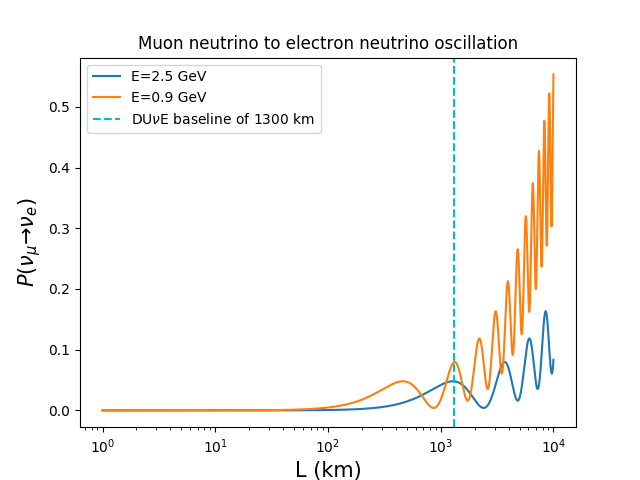
\includegraphics[width=0.48\textwidth,keepaspectratio]{numu-nue-vs-L-3flav.png}
            	\caption[$P(\nu_{\mu}\to\nu_e)$ en fonction de $L$]{$P(\nu_{\mu}\to\nu_e)$ en fonction de $L$. fonction de $L$ pour un neutrino de \SI{0.9}{\giga\electronvolt} et \SI{2.5}{\giga\electronvolt}. La ligne verticale représente la ligne de base de \gls{dune}. Le faisceau de neutrino envoyé aura des énergies allant de \SI{0.5}{\giga\electronvolt} et \SI{5}{\giga\electronvolt}, incluant donc les deux premiers maxima locaux de probabilité.}
            	\label{fig::3flavors_oscillations}
            \end{wrapfigure}
            Dans une expérience détectant des neutrinos, la probabilité sera moyennée sur le temps $t$, inconnu. Supposons que la source des neutrinos ait deux composantes d'énergies différentes $E_1$ et $E_2$, contribuant de manière cohérente au signal observé dans le détecteur. Au bout du temps $t$, chaque composante aura pris un facteur de phase $e^{-iE_jt}$. Les interférences entre les deux composantes feront alors entrer en jeu un facteur de phase $e^{-i(E_1-E_2)t}$. Moyenné sur $t$, ce facteur disparaît, sauf si $E_1 = E_2$. Les seules composantes contribuant de manière cohérente au signal ont donc une même énergie $E$. Ce point est détaillé dans les articles de Stodolsky\cite{Stodolsky1998}, Lipkin\cite{Lipkin2005} et Kayser\cite{Kayser2005}. On se retrouve donc avec l'équation suivante : 
            \begin{equation*}
                P(\nu_{\alpha}\to\nu_{\beta}) = \bigg|\sum_i U_{\alpha i}^*U_{\beta i} e^{-im_i^2\frac{L}{2E}}\bigg|^2.
            \end{equation*}
            Cette expression peut se mettre sous forme sinusoïdale\cite{Mondal2015} :
            \begin{equation}\label{eq::proba_oscillation}
                \begin{split}
                    P(\nu_{\alpha}\to\nu_{\beta}) = \delta_{\alpha\beta} & - 4\sum_{i>j}\Re(U_{\alpha i}U_{\beta i}^*U_{\alpha j}^*U_{\beta j})\sin^2\left(\Delta m_{ij}^2\frac{L}{4E}\right) \\
                    & +2\sum_{i>j}\Im(U_{\alpha i}U_{\beta i}^*U_{\alpha j}^*U_{\beta j})\sin\left(\Delta m_{ij}^2\frac{L}{2E}\right)
                \end{split}
            \end{equation}
            où $\Delta m_{ij}^2 = m_i^2-m_j^2$. Il peut être utile de définir une longueur d'oscillation $l_{osc} = 4\pi E/\Delta m_{ij}^2$ si l'on souhaite étudier les oscillations en fonction de la ligne de base $L$ pour des énergies fixées, réécrivant alors les termes en $\sin$ et $\sin^2$ :
            \begin{eqnarray}
                \sin^2\left(\Delta m_{ij}^2\frac{L}{4E}\right) = &  \sin^2\left(\pi\frac{L}{l_{osc}}\right) \\
                \sin\left(\Delta m_{ij}^2\frac{L}{2E}\right) = & \sin\left(2\pi\frac{L}{l_{osc}}\right).
            \end{eqnarray}
                        
            On peut noter trois choses:
            \begin{itemize}
                \item[$\bullet$] Le terme "oscillation" est ici évident : la probabilité qu'a un neutrinos de changer de saveur est une fonction sinusoïdale du ratio $\frac{L}{E}$. L'exemple du changement de saveur $P(\nu_{\mu}\to\nu_e)$, important pour les expériences comme \gls{dune} détectant des neutrinos issus de faisceaux, est illustré en \autoref{fig::3flavors_oscillations}.
                \item[$\bullet$] La masse d'un neutrino ne sera pas accessible par la mesure de probabilité d'oscillation : seule une différence de masse au carré est accessible. On ne peut donc pas, avec les oscillations des neutrinos, déterminer les valeurs des masses des neutrinos.
                \item[$\bullet$] Si les neutrinos ont des masses nulles ou égales, les termes en $\Delta m_{ij}^2$ s'annulent et les probabilités de transitions sont nulles. L'observation du phénomène d'oscillation des neutrinos montre donc bien que deux masses au moins sont non nulles.
                \item[$\bullet$] La somme $\sum_{\beta\in\{e,\mu,\nu\}}P(\nu_{\alpha}\to\nu_{\beta})$ doit être égale à 1 de par l'unitarité de $U$. Les neutrinos ne disparaissent pas entre leur émission et leur arrivée au détecteur\footnote{Leurs sections efficaces d'interaction sont trop faibles pour impacter le flux mesuré.}, ils changent de saveur. Mais si une de ces saveurs n'est pas observable parce que stérile, alors le flux total observable s'en verra diminué. Les résultats de SNO montrés en \autoref{fig::SNO_plot} tendent à montrer que la probabilité d'osciller vers un tel état est faible, au moins aux valeurs de $L/E$ correspondant aux neutrinos solaires.
            \end{itemize}
            
            On peut immédiatement calculer la même probabilité pour les antineutrinos, en supposant que la symétrie CPT n'est pas violée : 
            \begin{equation}
                P(\overline{\nu}_{\alpha}\to\overline{\nu}_{\beta}) = P(\nu_{\beta}\to\nu_{\alpha}).
            \end{equation}
            La partie réelle de l'équation \eqref{eq::proba_oscillation} restera inchangée, tandis que la partie imaginaire deviendra négative. On aura donc :
            \begin{equation}
                \begin{split}
                    P(\overline{\nu}_{\alpha}\to\overline{\nu}_{\beta}) = \delta_{\alpha\beta} & - 4\sum_{i>j}\Re(U_{\alpha i}U_{\beta i}^*U_{\alpha j}^*U_{\beta j})\sin^2\left(\Delta m_{ij}^2\frac{L}{4E}\right) \\
                    & -2\sum_{i>j}\Im(U_{\alpha i}U_{\beta i}^*U_{\alpha j}^*U_{\beta j})\sin\left(\Delta m_{ij}^2\frac{L}{2E}\right).
                \end{split}
            \end{equation}
            Et donc, si le dernier terme est différent de 0, les neutrinos et les antineutrinos se comportent différemment, montrant que la symétrie CP est brisée dans le modèle standard.
            
            Tous les calculs ont été fait en unités naturelles $\hbar = c = 1$. Il convient de repasser en unités SI si on veut pouvoir prédire des grandeurs mesurables. Une rapide analyse dimensionnelle montre que 
            \begin{eqnarray}
                \Delta m_{ij}^2\frac{L}{4E}(nat.)
                = \Delta m_{ij}^2\frac{L}{4E}\frac{c^3}{\hbar}(SI)
                \simeq \numprint{1.27}\Delta m_{ij}^2(\si{\electronvolt\squared})\frac{L(\si{\kilo\meter})}{E(\si{\giga\electronvolt})} \\ 
                l_{osc}(\si{\kilo\meter}) = \frac{4\pi E\hbar}{\Delta m_{ij}^2c^3} \simeq \numprint{2.48}\frac{E(\si{\giga\electronvolt})}{\Delta m_{ij}^2(\si{\electronvolt\squared})}.
            \end{eqnarray}
            
        \subsubsection{Deux cas particuliers}
            Deux cas particuliers et faciles à traiter sont les oscillations à deux saveurs, qui étaient de bonnes approximations pour les premières expériences de mesure de probabilité d'oscillation, et la probabilité de conservation, i.e $P(\nu_{\alpha}\to\nu_{\alpha})$.
            
            Commençons par le cas de conservation. L'équation \eqref{eq::proba_oscillation} nous donne :
            \begin{equation}\label{eq::proba_non_oscillation}
                \begin{split}
                    P(\nu_{\alpha}\to\nu_{\alpha}) = 1 & - 4\sum_{i>j}\Re(U_{\alpha i}U_{\alpha i}^*U_{\alpha j}^*U_{\alpha j})\sin^2\left(\Delta m_{ij}^2\frac{L}{4E}\right) \\
                    & + 2\sum_{i>j}\Im(U_{\alpha i}U_{\alpha i}^*U_{\alpha j}^*U_{\alpha j})\sin\left(\Delta m_{ij}^2\frac{L}{2E}\right) \\
                    = 1 & -4\sum_{i>j}\Re(|U_{\alpha i}|^2|U_{\alpha j}|^2)\sin^2\left(\Delta m_{ij}^2\frac{L}{4E}\right).
                \end{split}
            \end{equation}
            Le terme contenant la partie imaginaire de l'équation \eqref{eq::proba_oscillation} ayant disparu, cette probabilité sera la même pour les antineutrinos. Il n'est donc pas possible de mesurer l'asymétrie matière-antimatière avec cette probabilité. Le terme oscillant étant en $\sin^2$, il n'est pas possible non plus de déterminer le signe de $\Delta m_{ij}^2$ en mesurant cette probabilité.
            
            Le cas des oscillations à deux saveurs, correspondant à une probabilité négligeable d'osciller vers la troisième saveur, s'obtient facilement en fixant $n=2$. Dans ce cas la matrice $U$ est une simple matrice de rotation à deux dimensions, réelle, avec un paramètre $\theta$ :
            \begin{equation}\label{eq::two_flavor_pmns}
                U = \left(\begin{matrix}
                    \cos(\theta) & \sin(\theta) \\
                    -\sin(\theta) & \cos(\theta)
                \end{matrix}\right)
            \end{equation}
            et la probabilité \eqref{eq::proba_oscillation} devient
            \begin{eqnarray}
                \label{eq::two_flavors}
                P(\nu_{\alpha}\to\nu_{\beta}) = \sin^2(2\theta)\sin^2\left(\frac{\Delta m^2 L}{4E}\right) \\ 
                \label{eq::two_flavors_length}
                P(\nu_{\alpha}\to\nu_{\beta}) = \sin^2(2\theta)\sin^2\left(\pi\frac{L}{l_{osc}}\right) \\
                \label{eq::two_flavors_survival}
                P(\nu_{\alpha}\to\nu_{\alpha}) = 1- \sin^2(2\theta)\sin^2\left(\pi\frac{L}{l_{osc}}\right)
            \end{eqnarray}
            avec bien entendu $\alpha\ne \beta$ (il suffit de prendre 1 moins cette probabilité pour avoir la probabilité de conservation). Ici aussi, la violation de CP n'est pas accessible, il n'y aura pas de différence matière-antimatière. Due au carré du sinus, cette probabilité n'est pas sensible non plus au signe de $\Delta m^2$. Le terme en $\sin^2(2\theta)$ correspond à l'amplitude d'oscillation, c'est à dire la fraction maximale de neutrinos $\alpha$ pouvant se changer en neutrinos $\beta$. $l_{osc}$ correspond ici a la distance entre deux maxima ou minima de probabilité de transition.
            
            Dans quels cas cette approximation est-elle valide? Il se trouve que les mesures actuelles ont montré que la différence des masses carrés entre les deux premiers états propres est 300 fois plus faible que les deux autres : 
            \begin{equation}
                |\Delta m^2_{21}| << |\Delta m^2_{31}| \simeq |\Delta m^2_{32}|.
            \end{equation}
            De plus, un autre résultat est que le terme $U_{e3}$ est très petit devant 1. Ces deux résultats permettent dans de nombreux cas d'approximer les oscillations à trois saveurs par une oscillation à deux saveurs.
            
            La première approximation qui peut être faite est pratique pour les expériences de neutrinos atmosphériques, de réacteurs et d'accélérateurs à faible et moyenne ligne de base. Dans ces cas, $L/E$ vérifie
            \begin{equation}\label{eq::approx_21_0}
                \Delta m^2_{21}\frac{L}{2E} << 1.
            \end{equation}
            et tous les termes en $\sin$ et $\sin^2$ dépendant de $\Delta m^2_{21}$ tendent vers 0. La probabilité de transition $\nu_{\alpha}\to\nu_{\beta}$ devient alors
            \begin{equation}
                P(\nu_{\alpha}\to\nu_{\beta}) = 4|U_{\alpha 3}|^2|U_{\beta 3}|^2\sin^2\left(\Delta m^2_{31}\frac{L}{4E}\right).
            \end{equation}
            qui est exactement la probabilité de transition dans l'approximation à deux saveurs \eqref{eq::two_flavors} si l'on identifie $4|U_{\alpha 3}|^2|U_{\beta 3}|^2=\sin^2(2\theta)$.
            
            La seconde approximation est utile lors de l'étude des neutrinos solaires et des expériences à très longue ligne de base. Dans ces cas, $L/E$ est trop grand pour que \eqref{eq::approx_21_0} soit vraie. En revanche, les relations suivantes sont vérifiées : 
            \begin{equation}\label{eq::approx_31_eq_32}
                \Delta m^2_{31}\frac{L}{2E} \simeq \Delta m^2_{32}\frac{L}{2E}  >> 1.
            \end{equation}
            Dans ce cas les oscillations dues à $\Delta m^2_{31}$ et $\Delta m^2_{32}$ sont tellement rapides qu'elles donnent lieu à un effet moyen qui donne comme probabilité de survie du neutrino électronique
            \begin{equation}
                P(\nu_e\to\nu_e) \simeq \sin^4(\theta_{13}) + \cos^4(\theta_{13})\left(1-\sin^2(2\theta_{12})\sin^2\left(\Delta m^2_{21}\frac{L}{4E}\right)\right)
            \end{equation}
            où les angle $\theta_{13}$ et $\theta_{12}$ sont introduits dans la section suivante et correspondent à $\sin(\theta_{13})=U_{e3}$ et $\sin(\theta_{12})\cos(\theta_{13})=U_{e2}$.
            
            Il est immédiat alors que si l'approximation 
            \begin{equation}\label{eq::approx_13_eq_0}
                U_{e3} << 1
            \end{equation}
            est valide, l'équation précédente devient
            \begin{equation}\label{eq::solar_oscillation}
                P(\nu_e\to\nu_e) \simeq 1-\sin^2(2\theta_{12})\sin^2\left(\Delta m^2_{21}\frac{L}{4E}\right).
            \end{equation}
            qui correspond à la probabilité de survie à deux saveurs \eqref{eq::two_flavors_survival}.
            
            Ces différentes approximations ont été utilisées dans la plupart des expériences d'oscillation des neutrinos jusqu'à aujourd'hui. Le défi des expériences les plus récentes et des expériences futurs est d'être sensible aux effets au delà de ces approximations, car ces effets peuvent contenir de la physique au delà du modèle standard comme nous allons le voir plus tard.
            
        \subsection{La matrice PMNS}\label{sec::pmns}
            \subsubsection{Généralités}
            Il est temps de décrire un peu plus en détail la $U$, également appelé matrice \gls{pmns}. Elle est de la forme : 
            \begin{equation}
                \left(\begin{matrix}
                     \nu_e \\ \nu_{\mu} \\ \nu_{\tau} \\ ...
                \end{matrix}\right) =
                \underbrace{\left(\begin{matrix}
                    U_{e1} & U_{e2} & U_{e3} & ... \\
                    U_{\mu 1} & U_{\mu 2} & U_{\mu 3} & ... \\
                    U_{\tau 1} & U_{\tau 2} & U_{\tau 3} & ... \\
                    ... & ... & ... &
                \end{matrix}\right)}_U
                \left(\begin{matrix}
                     \nu_1 \\ \nu_2 \\ \nu_3 \\ ...
                \end{matrix}\right)
            \end{equation}
            où les pointillés soulignent le fait que cette matrice n'est pas forcément $3\times 3$. Cette matrice représente une matrice de changement de base, équivalente à une matrice de rotation complexe à $n$ dimensions. Une telle matrice peut se représenter comme un produit de $\frac{n}{2}(n-1)$ matrices de rotation dans un plan donné\cite{Valle2006,Harari1986} : 
            \begin{equation}\label{eq::compact_pmns}
                U=u_0(\gamma)\prod_{i<j}^n u_{ij}
            \end{equation}
            où $u_0(\gamma)=e^{i \sum_{i}^{n}\gamma_i \mathbb{I}}$ est une matrice diagonale unitaire arbitraire ($\gamma$ est un vecteur quelconque) et $u_{ij}$ est une matrice de rotation telle que
            \begin{equation}
                \begin{split}
                    u_{ij}= & e^{\sum_{i=1}^n\left(\eta_{ij}A_i^j-\eta_{ij}^*A_j^i\right)},\\
                    \eta_{ij} = & \theta_{ij}e^{i\phi_{ij}},\\
                    \left(A_i^j\right)_k^l = & \delta_{ik}\delta_{jl}.
                \end{split}
            \end{equation}
            
            Par exemple, la matrice de rotation dans la plan $12$ sera
            \begin{equation}
                u_{12} = 
                \left(\begin{matrix}
                    \cos(\theta_{12}) & e^{i\phi_{12}}\sin(\theta_{12}) & 0 & ... \\
                    -e^{-i\phi_{12}}\sin(\theta_{12}) & \cos(\theta_{12}) & 0 & ... \\
                    0 & 0 & 1 & ... \\
                    ... & ... & ... &
                \end{matrix}\right).
            \end{equation}
            Cette matrice aura alors $n^2$ paramètres réels, $\frac{n}{2}(n-1)$ angles  et $\frac{n^2+n}{2}$ phases.
            
            \subsubsection{La matrice PMNS à trois dimensions}
            Jusqu'ici nous avons considéré la matrice $U$ comme ayant une dimension de 3 ou plus, afin de considérer les éventuels neutrinos stériles. Dans la suite, nous supposerons que seuls 3 états de saveurs peuvent osciller entre eux. $U$ a alors 3 angles et 6 phases.
            
            Si nos neutrinos sont de Dirac, alors les champs des leptons chargés $l_{\alpha}$ et des états de masse des neutrinos $\nu_i$ peuvent être multipliés par une phase complexe\footnote{La phase affectant les champs de chiralité droite doit être opposée à celle affectant les champs de chiralité gauche afin de laisser invariant le terme de masse de Dirac \eqref{eq::dirac_mass}.} sans changer ni leurs lagrangiens libres ni leurs lagrangiens d'interaction. En d'autres termes, effectuer la transformation 
            \begin{eqnarray}
                l_{\alpha}\to & e^{i\phi_{\alpha}}l_{\alpha} \\
                \nu_i\to & e^{i\phi_i}\nu_i 
            \end{eqnarray}
            laisse la physique invariante. Un terme d'interaction lepton-neutrino comporte $\sum_{\alpha}\bar{l}_{\alpha L}\gamma^{\mu}\sum_i U_{\alpha i}\nu_{i L}$, où $\bar{l}_{\alpha L}$ est le conjugué de Dirac de $l_{\alpha L}$ et $\gamma^{\mu}$ sont les matrices de Dirac. On utilise cette liberté dans le choix des phases des champs pour redéfinir $U$ de la manière suivante :
            \begin{equation}
                U_{\alpha i}\to e^{i(\phi_{\alpha}-\phi_i)}U_{\alpha i}.
            \end{equation}
            
            $U$ est alors affectée par les différences de phase $(\phi_{\alpha}-\phi_i)$. Il y en a 5 indépendantes, qui peuvent absorber autant de phases de la matrice $U$, laissant une phase dans une des matrices $u_{ij}$. La paramétrisation utilisée par la communauté de la physique des neutrinos est celle qui place cette phase dans la matrice $u_{13}$.
            
            Si les neutrinos sont de Majorana, on ne peut pas rephaser le champ des états de masse des neutrinos. En effet, le terme de masse d'un neutrino de Majorana (voir équation \eqref{eq::majorana_mass}) deviendrait complexe. Seuls les 3 leptons chargés peuvent donc être rephasés, et donc seules 3 phases peuvent être absorbées. La paramétrisation de $U$ a laquelle nous aboutissons est alors la suivante, en notant $c_{ij}=\cos(\theta_{ij})$ et $s_{ij}=\sin(\theta_{ij})$: 
            \begin{eqnarray}
                U= & 
                \left(\begin{matrix}
                        1   &    0    &    0   \\
                        0   & c_{23}  & s_{23} \\
                        0   & -s_{23} & c_{23} \\
                \end{matrix}\right)\times
                \left(\begin{matrix}
                    c_{13}  &    0    & s_{13}e^{-i\delta_{CP}} \\
                        0   &    1    &    0   \\
    -s_{13}e^{i\delta_{CP}} &    0    & c_{13} \\
                \end{matrix}\right)\times
                \left(\begin{matrix}
                    c_{12}  & s_{12}  &    0   \\
                    -s_{12} & c_{12}  &    0   \\
   -                    0   &    0    &    1   \\
                \end{matrix}\right)\times
                \left(\begin{matrix}
              e^{i\alpha_1} &    0    &    0   \\
                        0   & e^{i\alpha_2} & 0 \\
                        0   & 0 & 1 \\
                \end{matrix}\right) \\\label{eq::pmns}
                =& 
                \left(\begin{matrix}
c_{12}c_{13}                                    & s_{12}c_{13}                                    & s_{13}e^{-i\delta_{CP}} \\
-s_{12}c_{23}-c_{12}s_{13}s_{23}e^{i\delta_{CP}} & c_{12}c_{23}-s_{12}s_{13}s_{23}e^{i\delta_{CP}} & c_{13}s_{23} \\
s_{12}s_{23}-c_{12}s_{13}c_{23}e^{i\delta_{CP}} & -c_{12}s_{23}-s_{12}s_{13}c_{23}e^{i\delta_{CP}} & c_{13}c_{23} \\
                \end{matrix}\right)\times
                \left(\begin{matrix}
              e^{i\alpha_1} &    0    &    0   \\
                        0   & e^{i\alpha_2} & 0 \\
                        0   & 0 & 1 \\
                \end{matrix}\right) .
            \end{eqnarray}
            La dernière matrice correspond aux phases restantes si les neutrinos sont de Majorana. Cette dernière n'a aucune influence sur les probabilités de changement de saveur. La phase dans la seconde matrice est appelée phase de violation CP, terme qui sera justifié dans la prochaine section. Dernière simplification : on peut choisir $\theta_{ij}\in [0;\frac{\pi}{2}]$ et $\delta_{CP}\in[0;2\pi[$.
            
            \subsubsection{Développement limité de la matrice PMNS et terme de violation CP}
            L'approximation \eqref{eq::approx_21_0} permet de simplifier certaines probabilités en les exprimant comme des oscillations à deux saveurs. Pour les expériences les plus récentes comme NO$\nu$A ou T2K (et \gls{dune} quand elle prendra des données), les sensibilités seront assez bonnes pour que cette approximation échoue à prédire précisément le spectre attendu. Il est en revanche possible d'utiliser des développements en série autour de $\alpha=\Delta m^2_{21}/\Delta m^2_{31}$ jusqu'à l'ordre 2 sans perdre en précision. Cette approche est valable pour des énergies supérieures ou égales au \si{\giga\electronvolt} et des lignes de bases inférieures à la dizaine de milliers de kilomètres\cite{Freund2001}, et est donc particulièrement utile pour les expériences de neutrinos d'accélérateurs. La probabilité la plus recherchée par ces expériences, à savoir $P(\nu_{\mu}\to\nu_e)$, s'écrit alors\cite{Giganti2017}
             : 
            \begin{equation}\label{eq::dvpt_3flavor_accelerator}
                \begin{split}
                P(\nu_{\mu}\to\nu_e) & \simeq  \sin^2(\theta_{23})\sin^2(2\theta_{13})\sin^2\left(\Delta m^2_{31}\frac{L}{4E}\right)
                + \cos^2(\theta_{23})\sin^2(2\theta_{12})\sin^2\left(\Delta m^2_{21}\frac{L}{4E}\right) \\ 
                & + \frac{1}{2}\cos(\theta_{13})\sin(2\theta_{12})\sin(2\theta_{13})\sin(2\theta_{23})\cos(\delta_{CP})\sin\left(\Delta m^2_{21}\frac{L}{4E}\right)\sin\left(\Delta m^2_{31}\frac{L}{2E}\right) \\
                & - \cos(\theta_{13})\sin(2\theta_{12})\sin(2\theta_{13})\sin(2\theta_{23})\sin(\delta_{CP})\sin\left(\Delta m^2_{21}\frac{L}{4E}\right)\sin^2\left(\Delta m^2_{31}\frac{L}{4E}\right)
                \end{split}
            \end{equation}
            Comme il est souligné dans \cite{Giganti2017}, on peut réécrire cette probabilité sous une forme plus compacte : 
            \begin{equation}
                P(\nu_{\mu}\to\nu_e) \simeq A^2_{atm} + A^2_{sol} + 2\cos(\theta_{13})A_{atm}A_{sol}\cos\left(\Delta m^2_{31}\frac{L}{4E} + \delta_{CP}\right)
            \end{equation}
            où $A_{atm} = \sin(\theta_{23})\sin(2\theta_{13})\sin\left(\Delta m^2_{31}\frac{L}{4E}\right)$ et $A_{sol} =\cos(\theta_{23})\sin(2\theta_{12})\sin\left(\Delta m^2_{21}\frac{L}{4E}\right)$. Le dernier terme sera sensible à la phase de violation CP, et on peut quantifier l'impact de cette violation sur l'oscillation $\nu_{\mu}\to\nu_e$ avec la grandeur
            \begin{equation}\label{eq::CP_A_factor}
                A_{\mu e} = \frac{P(\nu_{\mu}\to\nu_e)-P(\overline{\nu}_{\mu}\to\overline{\nu}_e)}{P(\nu_{\mu}\to\nu_e)+P(\overline{\nu}_{\mu}\to\overline{\nu}_e)} \simeq -\frac{\cos(\theta_{23})\sin(2\theta_{12})}{\sin(\theta_{23})\sin(\theta_{13})}\sin\left(\Delta m^2_{21}\frac{L}{4E}\right)\sin(\delta_{CP}).
            \end{equation}


    \section{Les effets de matières}\label{sec::matter_effect}
        Jusqu'à présent, nous n'avons parlé que des neutrinos oscillant dans le vide. En pratique, seulement très peu de cas y correspondent : les neutrinos issues du soleil ou de supernovae traversent des milieux très denses avant de se propager dans le vide, les neutrinos atmosphériques peuvent traverser la Terre avant d'être détectés, et les expériences de réacteur ou d'accélérateur à longue ligne de base détectent les neutrinos après qu'ils aient traversé la croûte terrestre.
        \subsection{Le cas à deux saveurs : illustration de l'effet Mikheyev-Smirnov-Wolfenstein}
            \subsubsection{Modification de l'Hamiltonien et nouveaux états propres}
            La première question à se poser est : comment les neutrinos interagissent-ils avec la matière? Seule la diffusion vers l'avant a un effet sur les oscillations\cite{Wolfenstein1978,Akhmedov2000} et résulte d'un potentiel $V_{\alpha}$, différent d'une saveur de neutrino à l'autre. Cette diffusion peut être induite par courant chargé (échange d'un boson $W^{\pm}$) entre un neutrino électronique et un électron, ou par un courant neutre (échange d'un boson $Z$) entre n'importe quelle saveur de neutrino et un proton, un neutron ou un électron.
            
            Le courant chargé est décrit, à basse énergie, par l'hamiltonien effectif\cite{Akhmedov2000}
            \begin{equation}
                H_{CC} = \frac{G_F}{\sqrt{2}}\left[\overline{e}\gamma_{\mu}(1-\gamma_5)e\right]\left[\overline{\nu}_e\gamma^{\mu}(1-\gamma_5)\nu_e\right].
            \end{equation}
            où $G_F$ est la constante de Fermi. Pour calculer l'effet de la diffusion vers l'avant, on peut fixer les états des neutrinos et intégrer sur les états des électrons : 
            \begin{equation}
                H_{eff}(\nu_e) = \left<H_{CC}\right>_{e} \equiv \overline{e}V_e\nu_e
            \end{equation}
            où $V_e$ correspond au potentiel $V_{\alpha}$ pour les neutrinos électroniques. Ce qui donne après calcul pour un milieu non polarisé et d'impulsion résultante nulle\cite{Akhmedov2000}
            \begin{equation}
                V_{e,CC} = V_{CC} = \sqrt{2}G_F N_e
            \end{equation}
            où $N_e$ est la densité d'électrons. Concernant les termes de courant neutre, les contributions des protons et des électrons s'annuleront si la matière est électriquement neutre, ce que l'on va supposer ici. Seule le terme des neutrons reste et s'écrit 
            \begin{equation}
                V_{\alpha,NC} = -\frac{G_F N_n}{\sqrt{2}}
            \end{equation}
            où $N_n$ est la densité de neutrons. On a alors 
            \begin{eqnarray}
                V_e = \sqrt{2}G_F\left(N_e-\frac{N_n}{2}\right), & V_{\mu} = V_{\tau} = -\frac{G_F N_n}{\sqrt{2}}.
            \end{eqnarray}
            Les signes des potentiels sont inversés dans le cas des antineutrinos.
            En l'absence de matière, les états propres de l'hamiltonien sont les états propres de masses et suivent l'équation
            \begin{equation}
                i\frac{d}{dt}\ket{\nu_i} = \left(\begin{matrix}E_1 & 0 \\ 0 & E_2\end{matrix}\right)\ket{\nu_i}.
            \end{equation}
            Dans la base des états de saveurs, l'équation d'évolution s'écrit alors
            \begin{equation}\label{eq::evolution_matter_2flavor}
                i\frac{d}{dt}\ket{\nu_{\alpha}} = U\left(\begin{matrix}E_1 & 0 \\ 0 & E_2\end{matrix}\right)U^{\dagger}\ket{\nu_{\alpha}}.
            \end{equation}
            Dans l'approximation ultra-relativiste on peut écrire $E_i \simeq p+ \frac{m_i^2}{2E}$. On peut effectuer un rephasage pour enlever les termes diagonaux égaux. En utilisant l'équation \eqref{eq::two_flavor_pmns}, on obtient alors :
            \begin{equation}
                i\frac{d}{dt}\left(\begin{matrix}\nu_e \\ \nu_{\mu}\end{matrix}\right) = \left(\begin{matrix}-\frac{\Delta m^2}{4E}\cos(2\theta_0) & \frac{\Delta m^2}{4E}\sin(2\theta_0) \\ \frac{\Delta m^2}{4E}\sin(2\theta_0) & \frac{\Delta m^2}{4E}\cos(2\theta_0)\end{matrix}\right)\left(\begin{matrix}\nu_e \\ \nu_{\mu}\end{matrix}\right)
            \end{equation}
            où $\nu_e$ et $\nu_{\mu}$ sont des amplitudes de probabilité dépendantes du temps. Pour avoir cette équation dans la matière, il faut rajouter aux termes diagonaux les potentiels $V_e$ et $V_{\mu}$. Ces termes ont en commun $-\frac{G_F N_n}{\sqrt{2}}$, qui correspond au courant neutre, et qui pourra donc être éliminé par rephasage global, de la même manière qui a permit d'éliminer 5 phases sur les 6 de la matrice PMNS. On se retrouve donc avec l'équation
            \begin{equation}\label{eq::hamiltonian_matter_2flavor}
                i\frac{d}{dt}\left(\begin{matrix}\nu_e \\ \nu_{\mu}\end{matrix}\right) = \underbrace{\left(\begin{matrix}-\frac{\Delta m^2}{4E}\cos(2\theta_0)+\sqrt{2}G_F N_e & \frac{\Delta m^2}{4E}\sin(2\theta_0) \\ \frac{\Delta m^2}{4E}\sin(2\theta_0) & \frac{\Delta m^2}{4E}\cos(2\theta_0)\end{matrix}\right)}_{H_m}\left(\begin{matrix}\nu_e \\ \nu_{\mu}\end{matrix}\right).
            \end{equation}
            Si on s'intéresse au cas de l'oscillation à deux saveur $\nu_e\rightleftharpoons\nu_{\tau}$, on a juste à remplacer les $\nu_{\mu}$ par des $\nu_{\tau}$. Dans le cas de l'oscillation $\nu_{\mu}\rightleftharpoons\nu_{\tau}$ en revanche, il n'y a pas de termes de courant chargé, et il n'y a donc pas de différence avec le cas dans le vide.
            
            La diagonalisation de $H_m$ donne des vecteurs propres et une nouvelle matrice de mélange s'écrivant :
            \begin{equation}
                 \left(\begin{matrix}\nu_A & \\ \nu_B\end{matrix}\right) = \left(\begin{matrix}\cos(\theta) & \sin(\theta) \\ -\sin(\theta) & \cos(\theta)\end{matrix}\right)\left(\begin{matrix}\nu_e \\ \nu_{\mu}\end{matrix}\right)
            \end{equation}
            avec 
            \begin{equation}\label{eq::tan2theta}
                \tan(2\theta)=\frac{\frac{\Delta m^2}{4E}\sin(2\theta_0)}{\frac{\Delta m^2}{4E}\cos(2\theta_0)-\sqrt{2}G_F N_e}.
            \end{equation}
            Comme $\theta$ et $\theta_0$ sont différents, ces nouveaux états propres de propagation dans la matière ne sont pas les mêmes que les états propres de propagation dans le vide. On les appellera états propres de matière. La différence des énergies propres $E_A$ et $E_B$ est alors de 
            \begin{equation}
                E_A - E_B = \sqrt{\left(\frac{\Delta m^2}{2E}\cos(2\theta_0)-\sqrt{2}G_F N_e\right)^2 + \left(\frac{\Delta m^2}{2E}\sin(\theta_0)\right)^2}.
            \end{equation}
            
            On peut alors calculer la probabilité de transition de  $\nu_e\to\nu_{\mu}$ : 
            \begin{equation}\label{eq::two_flavors_matter}
                P(\nu_e\to\nu_{\mu}) = \sin^2(2\theta)\sin^2\left(\pi\frac{L}{l_m}\right)
            \end{equation}
            avec $l_m=\frac{2\pi}{E_A-E_B}$ la longueur d'oscillation dans la matière. Cette probabilité a la même forme que celle dans le vide \eqref{eq::two_flavors}. Dans la limite où $Ne\to 0$, on a $l_m\to 4\pi E/\Delta m^2$ et $\theta \to \theta_0$, redonnant bien \eqref{eq::two_flavors}.
            
            \subsubsection{L'effet de résonance Mikheyev-Smirnov-Wolfenstein}
            La nouvelle amplitude d'oscillation $\sin^2(2\theta)$ s'écrit maintenant
            \begin{equation}
                \sin^2(2\theta) = \frac{\left(\frac{\Delta m^2}{2E}\sin(2\theta_0)\right)^2}{\left(\frac{\Delta m^2}{2E}\cos(2\theta_0) - \sqrt{2}G_F N_e\right)^2 + \left(\frac{\Delta m^2}{2E}\sin(2\theta_0)\right)^2}.
            \end{equation}
            
            \begin{wrapfigure}[22]{R}{0.5\textwidth}
            	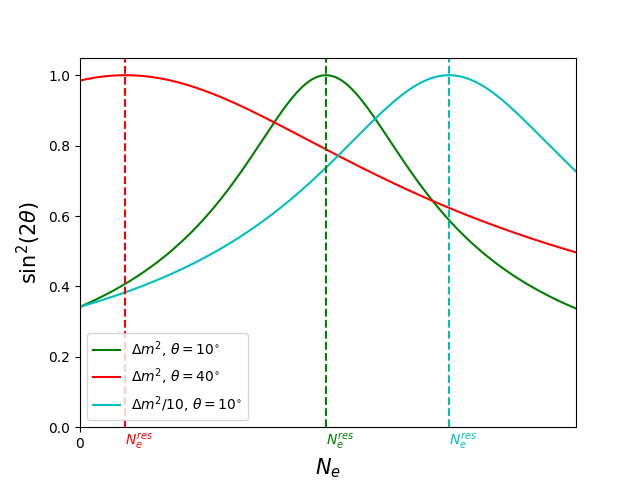
\includegraphics[width=0.5\textwidth,keepaspectratio]{msw_ne.png}
            	\caption[Effet de résonnance \gls{msw}]{\label{fig::amp_matter_vs_Ne}Amplitude de probabilité de changement de saveur de neutrinos se propageant dans la matière (approximation à deux saveur) en fonction de la densité d'électron $N_e$, pour différents angles de mélange dans le vide et différentes différence de masse au carré : il existe une valeur de $N_e$ où cette probabilité est de 1.}
            		%FAIRE un meilleur plot, où l'on voit les tendances à $\pm\infty$, et mettre $\theta_0$ dans le label au lieu de $\theta$.}
            \end{wrapfigure}
            Cette amplitude est représentée en fonction de la densité $N_e$ sur la \autoref{fig::amp_matter_vs_Ne}. On voit qu'elle a un maximum de 1 quand $N_e = N_e^{res}$ et qu'elle tend vers 0 à $\pm\infty$, et ce peu importe l'angle $\theta_0$. Autrement dit, même pour un très petit angle de mélange dans le vide, l'amplitude d'oscillation peut être de 1 si la densité d'électron dans le milieu traversé atteint une valeur de résonance
            \begin{equation}\label{eq::MSW_condition}
                N_e^{res}=\frac{\Delta m^2\cos(2\theta_0)}{2\sqrt{2}G_F E}.%=\numprint{6.56e6}\frac{\Delta m^2(\si{\electronvolt\squared})}{E(\si{\mega\electronvolt})}\cos(2\theta_0)N_A\si{\centi\meter^{-3}}
            \end{equation}
            %où $N_A$ est le nombre d'Avogadro.
            Cet effet, appelé effet \gls{msw}, doit être pris en compte dans les expériences de neutrinos solaires, où la densité décroît depuis le centre du soleil jusqu'à sa surface, dans le cas des neutrinos atmosphériques traversant la Terre, dont le profile de densité peut être vu comme une succession de différentes densités constantes, et dans les expériences à longue ligne de base de réacteur et d'accélérateur, où les électrons traversent la croûte terrestre, dont la densité est en bonne approximation constante.
            
            %Dans le cas des expériences à longue ligne de base de type réacteur ou accélérateur, la densité de matière correspond à celle de la croûte terrestre qui est globalement constante. En revanche, le spectre en énergie des neutrinos incidents peut être large, ce sera le cas notamment pour \gls{dune}. Il est donc plus pratique d'exprimer la condition \eqref{eq::MSW_condition} de la manière suivante : 
            %\begin{equation}
            %    E^{res}=\frac{\Delta m^2\cos(2\theta_0)}{2\sqrt{2}G_F N_e}=\numprint{6.56e6}\frac{\Delta m^2(\si{\electronvolt\squared})}{N_e(N_A\si{\centi\meter^{-3}})}\cos(2\theta_0)(\si{\mega\electronvolt}).
            %\end{equation}
            
            Deux choses sont à noter : 
            \begin{itemize}
            	\item[$\bullet$] Les effets de matière sont sensibles au signes de $\Delta m^2$.
                \item[$\bullet$] Il y a une condition à remplir pour que cette résonance soit possible : il faut que $\frac{\Delta m^2}{2E}\cos(2\theta_0) > 0$ dans le cas des neutrinos et $\frac{\Delta m^2}{2E}\cos(2\theta_0) < 0$ dans le cas des antineutrinos, puisqu'une densité ne peut être négative. Il ne peut donc pas y avoir de résonance à la fois pour les neutrinos \textit{et} pour les antineutrinos. Cet effet induit donc une violation de CP macroscopique dans l'observation des oscillations dans la matière, qui n'a rien à voir avec la phase de violation de CP de la matrice PMNS, et qu'il convient de modéliser précisément pour toute tentative de mesure de $\delta_{CP}$.
                \item[$\bullet$] Si l'angle de mélange dans le vide est strictement nul, il ne peut pas y avoir de résonance. En effet, dans ce cas, l'équation \eqref{eq::tan2theta} donne $\tan(2\theta)=0$ et donc $\theta=\frac{\pi}{2}$, rendant les états propres de saveurs orthogonaux et donc non-mélangeables.
                \item[$\bullet$] Si $N_e$ est variable le long du parcours des neutrinos, ce qui est le cas des neutrinos solaires ou des neutrinos passant par le centre de la Terre, la résonance est atteinte si au moins une région à un $N_e$ satisfaisant \eqref{eq::MSW_condition}. Ces cas ne correspondant pas aux expériences de neutrinos d'accélérateurs à longue ligne de base, aussi nous ne les détaillons pas. Un traitement de ces cas peut être trouvé ici \cite{Akhmedov2000}.
                \item[$\bullet$] Si les neutrinos ont un spectre en énergie relativement large, la résonance ne peut être atteinte que par une certaine partie du spectre seulement.
                \item[$\bullet$] En pratique, pour une source de neutrinos donnée, l'effet \gls{msw} se manifestera pour deux régions d'énergie, correspondant à la condition \eqref{eq::MSW_condition} satisfaite avec $\Delta m^2_{21}$ ou $\Delta m^2_{31}\simeq\Delta m^2_{32}$.
            \end{itemize}
                
            
        \subsection{Le cas à trois saveurs}\label{sec::3flavor_matter}
            Le calcul des effets de matière à trois saveurs suit la même logique que le cas à deux saveurs : il faut définir un nouvel Hamiltonien comme dans l'équation \eqref{eq::hamiltonian_matter_2flavor} et le diagonaliser pour trouver les nouveaux vecteurs et valeurs propres et la matrice de mélange dans la matière. Les calculs sont effectués en détails par Freund \cite{Freund2001}. Un point est à souligner : le calcul des vecteurs et valeurs propres s'effectue par développement en série, autour de $\alpha=\Delta m^2_{21}/\Delta m^2_{31}$. Il en ressort deux résultats possibles, suivant que le paramètre $\hat{A}=\frac{2V_{CC}E}{\Delta m^2_{31}}$ est petit ou non, qui correspondent aux deux résonances \gls{msw} possibles, à savoir la résonance solaire quand $\hat{A}=\alpha\simeq\numprint{0.03}$ et la résonance atmosphérique quand $\hat{A}=\cos(2\theta_{13})\simeq \numprint{0.95}$. C'est cette dernière qui est valable pour l'expérience \gls{dune}, qui fait entrer en jeu la densités de matière de la croûte terrestre, qui a une ligne de base inférieure à la dizaine de milliers de kilomètres et des énergies supérieures à \SI{0.35}{\giga\electronvolt}\cite{Giganti2017}, .
            
            En prenant en compte les effets de matière, la probabilité $P(\nu_{\mu}\to\nu_e)$ développée dans l'équation \eqref{eq::dvpt_3flavor_accelerator}, qui est d'intérêt pour les expériences de neutrinos d'accélérateurs, devient alors\cite{Giganti2017}
            \begin{equation}\label{eq::proba_matter_3flavors}
	            \begin{split}
	            P(\nu_{\mu}\to\nu_e) & \simeq  \sin^2(\theta_{23})\frac{\sin^2(2\theta_{13})}{(\textcolor{blue}{A}-1)^2}\sin^2\left[(\textcolor{blue}{A}-1)\Delta_{31}\right]
	            + \alpha^2\cos^2(\theta_{23})\frac{\sin^2(2\theta_{12})}{\textcolor{blue}{A}^2}\sin^2\left(A\Delta_{31}\right) \\ 
	            & + \alpha\frac{\cos(\theta_{13})\sin(2\theta_{12})\sin(2\theta_{13})\sin(2\theta_{23})\cos(\textcolor{red}{\delta_{CP}})}{\textcolor{blue}{A}(1-\textcolor{blue}{A})}\cos\left(\Delta_{31}\right)\sin\left(A\Delta_{31}\right)\sin\left[(1-\textcolor{blue}{A})\Delta_{31}\right] \\
	            & - \alpha\frac{\cos(\theta_{13})\sin(2\theta_{12})\sin(2\theta_{13})\sin(2\theta_{23})\sin(\textcolor{red}{\delta_{CP}})}{\textcolor{blue}{A}(1-\textcolor{blue}{A})}\sin\left(\textcolor{blue}{\Delta_{31}}\right)\sin\left(A\Delta_{31}\right)\sin\left[(1-\textcolor{blue}{A})\Delta_{31}\right]
	            \end{split}
            \end{equation}
            où $\Delta_{31}=\Delta m^2_{31}\frac{L}{4E}$, $\alpha=\Delta m^2_{21}/\Delta m^2_{31}\simeq 0.03$  et $A=2V_{CC}E/\Delta m^2_{31}=2\sqrt{2}G_F N_eE/\Delta m^2_{31}$. Les éléments en bleu indiquent les occurrences de $A$ qui auront un impact différent sur $P(\overline{\nu}_{\mu}\to\overline{\nu}_e)$ suivant le signe de $\Delta m^2_{31}$, encore inconnu et important pour la détermination de la hiérarchie de masse (voir \autoref{sec::hierarchy}). Les éléments en rouges sont sensibles à la valeur de la phase de violation de CP. Le premier terme, où $\alpha$ n'apparaît pas, est dominé par $\Delta m^2_{31}$. Le second terme, fortement supprimé par $\alpha^2$, est dominé par $\Delta m^2_{21}$. Pour avoir la probabilité $P(\overline{\nu}_{\mu}\to\overline{\nu}_e)$, il faut alors inverser le signe de $\delta_{CP}$ et de $A$. Changer le signe de $\delta_{CP}$ change le signe du dernier terme, en $\sin(\delta_{CP})$, alors que changer le signe de $A$ aura une influence sur tous les termes sauf le second.
            
            Les expériences cherchant à mesurer une différence entre $P(\nu_{\mu}\to\nu_e)$ et $P(\overline{\nu}_{\mu}\to\overline{\nu}_e)$ afin de déterminer $\delta_{CP}$ devront donc favoriser les plus faibles lignes de bases, afin de s'affranchir des effets de matières (c'est ce que fait T2K et ce que fera Hyper-Kamiokande). A l'inverse, une très longue ligne de base est préférable pour les mesures du signe de $\Delta m^2_{31}$ (c'est ce que fait NO$\nu$A et ce que fera \gls{dune}), mais la sensibilité à $\delta_{CP}$ en sera diminuée. A noter qu'il est théoriquement possible de mesurer $\delta_{CP}$ et le signe de $\Delta m^2_{31}$ en étudiant uniquement $P(\nu_{\mu}\to\nu_e)$ étant donné que les valeurs de $A$ et $\delta_{CP}$ ont un impact direct sur $P(\nu_{\mu}\to\nu_e)$.

            %Dans le cas à trois saveurs, l'équation \eqref{eq::evolution_matter_2flavor} devient, en prenant en compte le potentiel $V_{CC}$ :
            %\begin{equation}\label{eq::evolution_matter_3flavor}
             %   i\frac{d}{dt}\left(\begin{matrix}\nu_e \\ \nu_{\mu} \\ \nu_{\tau}\end{matrix}\right) = \left [ \frac{1}{2E}U\underbrace{\left(\begin{matrix} m_1^2 & 0 & 0 \\ 0 & m_2^2 & 0 \\
              %  0 & 0 & m_3^2\end{matrix}\right)}_{M^2}U^{\dagger} + \left(\begin{matrix}V_{CC} & 0 & 0 \\ 0 & 0 & 0 \\ 0 & 0 & 0\end{matrix}\right)\right]\left(\begin{matrix}\nu_e \\ \nu_{\mu} \\ \nu_{\tau}\end{matrix}\right)
            %\end{equation}
            
            %\subsubsection{Justification de l'approximation à deux saveurs}
            %Si l'approximation \eqref{eq::approx_21_0} est valide, il est utile d'effectuer la transformation 
            %\begin{equation}
             %   M^2\to \widetilde{M}^2 = M^2-m_1^2\mathbb{I}=\left(\begin{matrix} 0 & 0 & 0 \\ 0  & \Delta m^2_{21} & 0 \\ 0 & 0 & \Delta m^2_{31}\end{matrix}\right) \simeq \left(\begin{matrix} 0 & 0 & 0 \\ 0  & 0 & 0 \\ 0 & 0 & \Delta m^2_{31}\end{matrix}\right)
            %\end{equation}
            %où le terme $m_1^2\mathbb{I}$ peut être absorbé par rephasage dans l'équation \eqref{eq::evolution_matter_3flavor}. Cette matrice commute avec $u_{12}$. En notant $V=\text{diag}(V_{CC},0,0)$, qui commute avec $u_{23}$, et $ \widetilde{\nu} = u_{23}\left(\nu_e, \nu_{\mu}, \nu_{\tau}\right)^T$, on obtient donc
            %\begin{eqnarray}
             %   & i\frac{d}{dt}\widetilde{\nu} = \left(\frac{1}{2E}u_{13}\widetilde{M}^2u^{\dagger}_{13} + V\right)\widetilde{\nu} \\ 
              %  \Rightarrow & i\frac{d}{dt}\left(\begin{matrix}\widetilde{\nu_a} \\ \widetilde{\nu_b} \\ \widetilde{\nu_c}\end{matrix}\right) = \left(\begin{matrix}  \frac{\Delta m^2_{31}}{2E}s^2_{13}+V_{CC} & 0 & \frac{\Delta m^2_{31}}{2E}s_{13}c_{13} \\ 0  & 0 & 0 \\ \frac{\Delta m^2_{31}}{2E}s_{13}c_{13} & 0 & \frac{\Delta m^2_{31}}{2E}c^2_{13} \end{matrix}\right)\left(\begin{matrix}\widetilde{\nu_a} \\ \widetilde{\nu_b} \\ \widetilde{\nu_b}\end{matrix}\right)
            %\end{eqnarray}
            %où $\widetilde{\nu_a} = \nu_e$ et $\widetilde{\nu_c} = s_{23}\nu_{\mu} + c_{23}\nu_{\tau}$.
            %Le problème se réduit donc à un problème d'oscillation à deux saveurs entre $\widetilde{\nu_a}$ et $\widetilde{\nu_b}$ où, après un dernier rephasage, on peut écrire
            %\begin{equation}
            %    i\frac{d}{dt}\left(\begin{matrix}\widetilde{\nu_a} \\ \widetilde{\nu_b}\end{matrix}\right) = \left(\begin{matrix} -\frac{\Delta m^2_{31}}{4E}\cos(2\theta_{13}) + \frac{V_{CC}}{2} & \frac{\Delta m^2_{31}}{4E}\sin(2\theta_{13}) \\ 
           %     \frac{\Delta m^2_{31}}{4E}\sin(2\theta_{13}) & \frac{\Delta m^2_{31}}{4E}\cos(2\theta_{13}) - \frac{V_{CC}}{2}\end{matrix}\right)\left(\begin{matrix}\widetilde{\nu_a} \\ \widetilde{\nu_b}\end{matrix}\right).
           % \end{equation}
            %\subsubsection{Approximation pour les expériences de neutrinos d'accélérateurs à longue ligne de base}

    \section{État de l'art}
    
	    \subsection{Les connaissances actuelles}
	   
		   \begin{table}[!h]
		   	\centering
		   	\begin{tabular*}{\textwidth}{@{\extracolsep{\fill}}|r||lclcl|} 
		   		\hline
		   		\textbf{Type d'expérience}            & $\mathbf{L}$ \textbf{[m]}  & & $\mathbf{E}$ \textbf{[MeV]}   & & $\mathbf{\Delta m^2}$ \textbf{[eV$^2$]}   \\ 
		   		\hline
		   		\hline
		   		Solaire                       & \numprint{e11}               & &1                          & &\numprint{e-11}             \\ 
		   		Atmosphérique                 & \numprint{e4} -- \numprint{e7}    & &\numprint{e2} -- \numprint{e5}       & &\numprint{e-1} -- \numprint{e-4} \\ 
		   		Réacteur                     & \numprint{e2} -- \numprint{e6}    & &1                          & &\numprint{e-2} -- \numprint{e-3} \\ 
		   		Accélérateur                 & \numprint{e2}                & &\numprint{e3} -- \numprint{e4}       & &$\gtrsim \numprint{0.1}$          \\ 
		   		Accélérateur à longue ligne de base   & \numprint{e5} -- \numprint{e6}    & &\numprint{e4}                   & &\numprint{e-2} -- \numprint{e-3} \\
		   		\hline
		   	\end{tabular*}
		   	\caption[Valeurs de $L$ et $E$ pour différents types d'expériences.]{Valeurs de $L$ et $E$ pour différents types d'expériences et valeur mesurables de $\Delta m^2$.}
		   	\label{tab::carac-experiments}
		   \end{table} 
	   
		    Il existe plusieurs sources capables de nous donner des renseignements sur les oscillations des neutrinos. La nature des informations accessibles dépend principalement des énergies $E$ et des lignes de base $L$. Le \autoref{tab::carac-experiments} présente ces différentes grandeurs pour les types d'expériences présentés ci-dessous, et précise les valeurs de $\Delta m^2$ mesurables.
		    
		    	\begin{figure}[htpb]
		    		\centering
		    		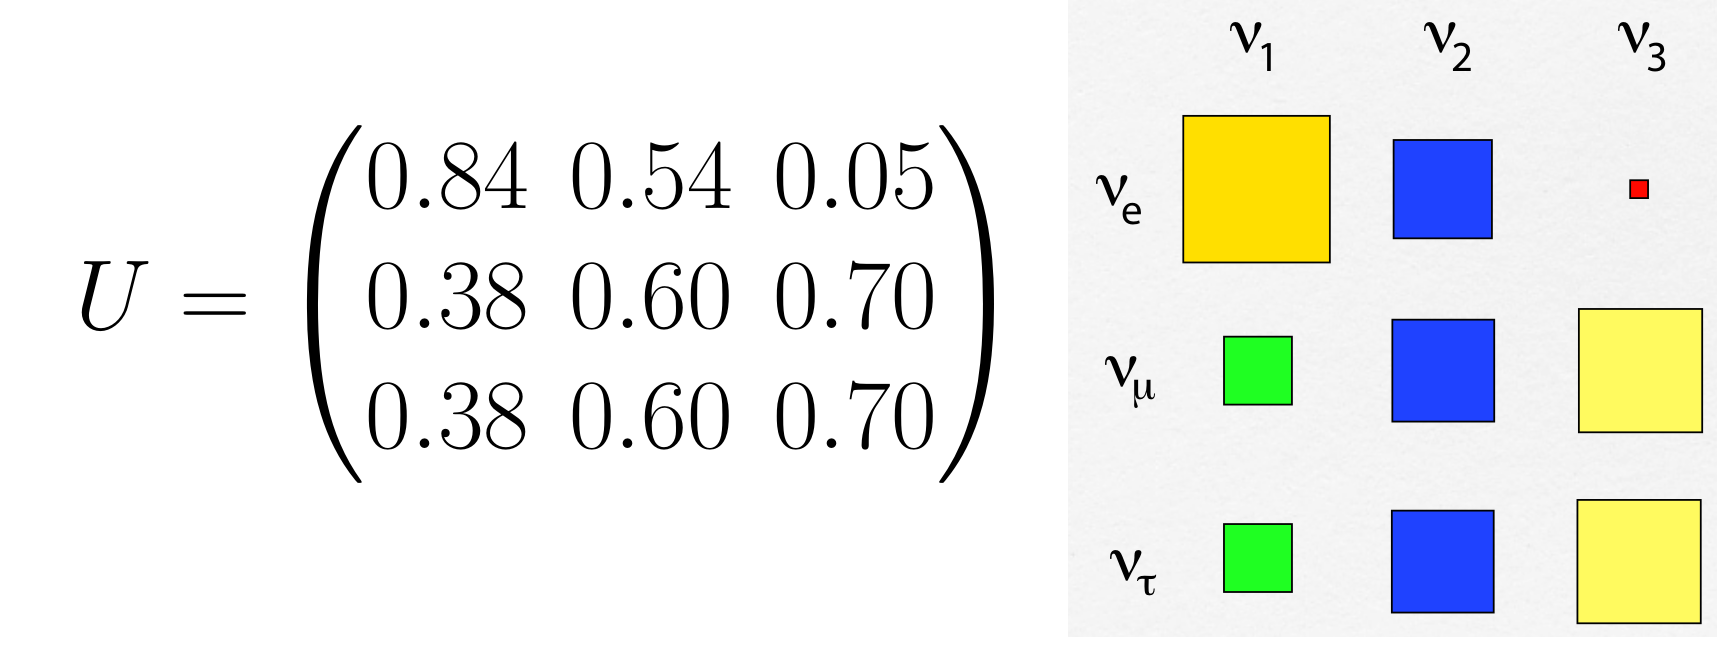
\includegraphics[width=.8\textwidth,keepaspectratio]{pmns.png}
		    		\caption[La matrice PMNS.]{Coefficients de la matrice PMNS. Image tirée de \cite{King2015}. Contrairement à la matrice CKM de mélange des quarks, qui est presque diagonale, le mélange des saveurs est très important dans le secteur leptonique.}
		    		\label{fig::pmns}
		    	\end{figure}
		    
		     Il y a des sources naturelles :
		    \begin{itemize}
		    	\item[$\bullet$] Les neutrinos solaires, issus des réactions de fusion nucléaire au coeur du soleil, sont des $\nu_e$ à leur création mais un certain nombre auront oscillé vers une autre saveur en quittant le soleil dû aux effets de matière décrits en \autoref{sec::matter_effect}. Plusieurs réactions entrent en jeu, chacune produisant des neutrinos d'énergies différentes et à des flux différents. %La figure \autoref{fig::solar_flux} montre les prédictions de ces flux par le Modèle Solaire Standard\cite{Bahcall2005}. 
		    	Ces neutrinos sont caractérisés par une énergie assez basse (de l'ordre du \si{\mega\electronvolt}) mais une ligne de base très longue, à savoir la distance Terre-Soleil.
		    	\item[$\bullet$] Les neutrinos atmosphériques, issus de la désintégrations de mésons et muons produits par les interactions des rayons cosmiques avec l'atmosphère, peuvent être à leur création des $\nu_{\mu}$, $\overline{\nu}_{\mu}$, $\nu_e$ et $\overline{\nu}_e$. Ils ont une énergie comprise entre 1 et $\SI{e5}{\giga\electronvolt}$ et une ligne de base allant de \SI{15}{\kilo\meter} pour les neutrinos arrivant du haut à \SI{12000}{\kilo\meter} pour ceux arrivant de l'autre côté du globe. Ces neutrinos subissent les effets de matière en traversant la Terre. Il est donc possible, pour une même source de neutrinos, de couvrir un large spectre de $L/E$. %La figure \autoref{fig::atm_flux} montre le spectre en énergie de ces neutrinos.
		    \end{itemize}
		    
		    et des sources artificielles:
		    \begin{itemize}
		    	\item[$\bullet$] Les neutrinos de réacteurs, issus des réactions de fissions au cœur des réacteurs nucléaires, sont des $\overline{\nu}_e$, avec un spectre en énergie allant de 1 à \SI{10}{\mega\electronvolt}.
		    	% montré en figure \autoref{fig::reactor_flux}. 
		    	L'avantage de ces expériences est qu'il est possible, dans une certaine limite, de choisir la ligne de base afin d'optimiser une oscillation autour d'un $\Delta m^2$ en fixant une valeur de $1.27\Delta m^2\frac{L}{E}$ proche de $\pi/2+n\pi$ afin de maximiser le terme en $\sin^2(1.27\Delta m^2\frac{L}{E})$.
		    	\item[$\bullet$] Les neutrinos d'accélérateurs, issus de faisceaux produit par l'homme, sont des $\nu_{\mu}$ (voir \autoref{sec::faisceau}). L'énergie est ajustable et le spectre peut être choisi de manière à être très piqué autour d'une valeur, comme dans l'expérience T2K, en plaçant la détecteur légèrement hors de l'axe du faisceau\cite{McDonald2001}, ou large, afin de couvrir plusieurs pics de $1.27\Delta m^2\frac{L}{E}=\pi/2+n\pi$. Ce sera le cas pour la future expérience \gls{dune}. De plus, la ligne de base est également ajustable.
		    \end{itemize}
		    Dans les deux cas de sources artificielles, si la ligne de base est grande, les neutrinos traverseront nécessairement la croûte terrestre et des effets de matière entreront alors en jeu.
		    
		    \begin{table}[!t]
		    	\centering
		    	\begin{tabular*}{\textwidth}{@{\extracolsep{\fill}}|r|cc|}
		    		\hline
		    		\textbf{Paramètre} & \textbf{meilleur ajustement} & \textbf{3}$\mathbf{\sigma}$  \\
		    		\hline
		    		\hline
		    		$\Delta m^2_{21}~[\SI{e-5}{\electronvolt\squared}]$ & \numprint{7.37}   & \numprint{6.93}--\numprint{7.96}\\
		    		$|\Delta m^2_{31}|~[\SI{e-3}{\electronvolt\squared}]$ & \numprint{2.56}   & \numprint{2.45}--\numprint{2.69} \\
		    		$\sin^2\theta_{12}$ & \numprint{0.297}   & \numprint{0.250}--\numprint{0.354}\\
		    		$\sin^2\theta_{23}$, $\Delta m^2_{31(23)}>0$ & \numprint{0.425}   & \numprint{0.381}--\numprint{0.615}\\
		    		$\sin^2\theta_{23}$, $\Delta m^2_{31(23)}<0$ & \numprint{0.589}   & \numprint{0.384}--\numprint{0.636}\\
		    		$\sin^2\theta_{13}$, $\Delta m^2_{31(23)}>0$ & \numprint{0.0215}   & \numprint{0.0190}--\numprint{0.0240}\\
		    		$\sin^2\theta_{13}$, $\Delta m^2_{31(23)}<0$ & \numprint{0.0216}   & \numprint{0.0190}--\numprint{0.0242}\\
		    		$\delta_{CP}/\pi$, $\Delta m^2_{31(23)}>0$ & \numprint{1.38} & $2\sigma$ :\numprint{1.0}--\numprint{1.9} \\
					\hline
		    	\end{tabular*}
		    	\caption[Meilleurs ajustements des mesures des paramètres des oscillations des neutrinos.]{\label{tab::pmns_values}Meilleurs ajustements des mesures des paramètres des oscillations, tiré la version de 2018 du PDG\cite{pdg2018}. Les incertitudes sont données à $3\sigma$, sauf pour $\delta_{CP}$ où elles sont données à $2\sigma$.}
		    \end{table}
		    
		    Les premières mesures de neutrinos atmosphériques, faites par Super-Kamiokande\cite{Fukuda1998}, ont montré que le flux des neutrinos électroniques ne présentait pas particulièrement d'excès ni de déficit, contrairement aux neutrinos muoniques. La probabilité de survie de ces derniers, en utilisant les approximations \eqref{eq::approx_21_0} et \eqref{eq::approx_13_eq_0}, s'écrit
		    \begin{equation}\label{eq::mu_approx_atmo}
		    P(\nu_{\mu}\to\nu_{\mu}) = 1 - \sin^2(2\theta_{23})\sin^2\left(\Delta m^2_{31}\frac{L}{4E}\right).
		    \end{equation}
		    De ce fait, la matrice $u_{23}$ est appelée matrice du "secteur atmosphérique". Ce secteur est également accessible grâce aux expériences de neutrinos d'accélérateurs à longue ligne de base, décrites plus en détail au chapitre suivant. Les principales expériences de neutrinos d'accélérateurs ayant fourni des résultats dans le secteur atmosphérique sont K2K\cite{Collaboration2006a}, T2K\cite{Abe2018}, NO$\nu$A\cite{Adamson2016} et MINOS\cite{Collaboration2014}. La mesure la plus précise à ce jour, issue d'un ajustement global des données actuelles, donne à $3\sigma$ $\sin^2(\theta_{23})=\numprint{0.425}^{+\numprint{0.19}}_{-\numprint{0.044}}$\cite{pdg2018} si la hiérarchie de masse est normale (voir \autoref{sec::hierarchy}), $\sin^2(\theta_{23})=0.589^{+0.047}_{-0.205}$ si elle est inversée. Ceci correspond à $\theta_{23}\simeq\SI{41}{\degree}$ si la hiérarchie est normale, et $\theta_{23}\simeq\SI{50}{\degree}$ si elle est inversée.
		    
		    Les approximations \eqref{eq::approx_31_eq_32} et \eqref{eq::approx_13_eq_0}, donnant la probabilité de survie des neutrinos électroniques venus du soleil \eqref{eq::solar_oscillation}, justifie que la matrice $u_{12}$ soit appelée matrice du "secteur solaire". Elle fut la première a être étudiée, surtout par Homesteak\cite{Lande1990}, SAGE\cite{Collaboration2009}, Gallex/GNO\cite{Hampel1999}, et plus tard par SNO\cite{Aharmim2013},  Kamiokande-II\cite{Hirata1992}, Super-Kamiokande\cite{Abe2018} et Borexino\cite{Collaboration2013}. KamLand\cite{Collaboration2004}, une expérience de neutrino de réacteur, a également fournit des informations sur le secteur solaire. La mesure la plus précise à ce jour, issue d'un ajustement global des données actuelles donne $\sin^2(\theta_{12})=\numprint{0.297}^{+\numprint{0.057}}_{-\numprint{0.047}}$\cite{pdg2018}, correspondant à $\theta_{12}\simeq\SI{33}{\degree}$, où les incertitudes correspondent à $3\sigma$.
		    
		    Les approximations \eqref{eq::approx_21_0} et \eqref{eq::approx_13_eq_0} donnent $P(\overline{\nu}_e\to\overline{\nu}_e) = 1-\sin^2(2\theta_{13})\sin^2\left(\Delta m^2_{31}\frac{L}{4E}\right)$ comme probabilité de survie des antineutrinos électroniques, approximations valables pour les expériences de neutrinos de réacteurs. Ceci justifie que la matrice $u_{13}$ soit appelée matrice du "secteur réacteur". La petite valeur de $\theta_{13}$ (inférieur à $\SI{10}{\degree}$) le rend plus difficilement mesurable. Les mesures des termes solaires et atmosphériques ont permis de déterminer qu'avec une ligne de base d'environ \SI{2}{\kilo\meter}, un détecteur proche d'un réacteur pouvait mesurer $\theta_{13}$, ce qui a été fait par Double Chooz\cite{Crespo-Anadon2014}, Reno\cite{Collaboration2010} et Daya Bay\cite{An2014}. Les expériences de neutrinos d'accélérateur à longue ligne de base K2K\cite{Collaboration2006a}, MINOS\cite{Collaboration2014} et T2K\cite{Abe2018} ont également fourni des résultats concernant $\theta_{13}$. La mesure la plus précise à ce jour, issue d'un ajustement global des données actuelles donne à $3\sigma$ $\sin^2(\theta_{13})=\numprint{0.0215}^{+\numprint{0.025}}_{-\numprint{0.025}}$\cite{pdg2018} si la hiérarchie de masse est normale (voir \autoref{sec::hierarchy}), $\sin^2(\theta_{13})=\numprint{0.0216}^{+\numprint{0.026}}_{-\numprint{0.026}}$ si elle est inversée. Ceci correspond à $\theta_{13}\simeq\SI{8.44}{\degree}$.
		    
		    \subsection{Ce qu'il reste à découvrir}
		    
			    La découverte des oscillations des neutrinos soulève beaucoup de questions, comme : pourquoi sont-ils aussi légers? Quelle est l'origine de leurs masses? Pourquoi deux différences de masse au carré sont si proches? Les neutrinos sont-ils de Dirac ou de Majorana? La matrice PMNS à 3 dimensions est-elle unitaire? Les neutrinos violent-ils la symétrie CP? Quelle est la hiérarchie de leur masse? Parmi toutes ces question, l'expérience \gls{dune} traitera essentiellement les deux dernières, détaillées maintenant.
		    
%		        \subsubsection{La matrice PMNS à plus de trois dimensions}
%		        
%	            Il n'est pas possible de généraliser brutalement l'expression \eqref{eq::pmns} à $n>3$ dimensions sans perdre en sens physique. En effet, $n$ dimensions implique $n$ types de neutrinos, et $n$ leptons chargés, mais ces derniers sont au nombre de 3.
%	            
%	            Que se passe-t-il si il existe plus de 3 neutrinos? Tout d'abord, ils ne peuvent pas interagir via l'interaction faible, comme nous l'avons mentionné plus haut. Ils ne se couplent donc pas aux leptons chargés. Même dans le cas où ces neutrinos sont de Dirac, nous ne pourrons plus éliminer autant de phases qu'avant. En effet, même si il existe $n$ neutrinos, il n'existe quand même que 3 leptons chargés, et donc il n'y a toujours que 5 phases qui pourront s'annuler, laissant dans la matrice $U$ un total de $2n-5$ phases similaires à $\delta_{CP}$. Si les neutrinos sont de Majorana, il y aura alors $n-1$ phases de Majorana.
%	            
%	            Si il existe plus de 3 saveurs de neutrinos pouvant se mélanger, alors la matrice PMNS ne devrait pas être unitaire. C'est en testant cette unitarité que l'on peut déterminer la dimension de la matrice. Un article de 2018\cite{Qian2013} décrit comment réaliser un tel test, qui requière plus de données que ce que l'on a actuellement pour donner un résultat précis. Pour le moment, les données sont compatibles avec une matrice PMNS à trois dimensions unitaire, et pose une limite sur les couplages avec un possible quatrième neutrino.
	            
	        
		        \subsubsection{La hiérarchie de masse}\label{sec::hierarchy}
		        
		        \begin{wrapfigure}{R}{0.5\textwidth}
		        	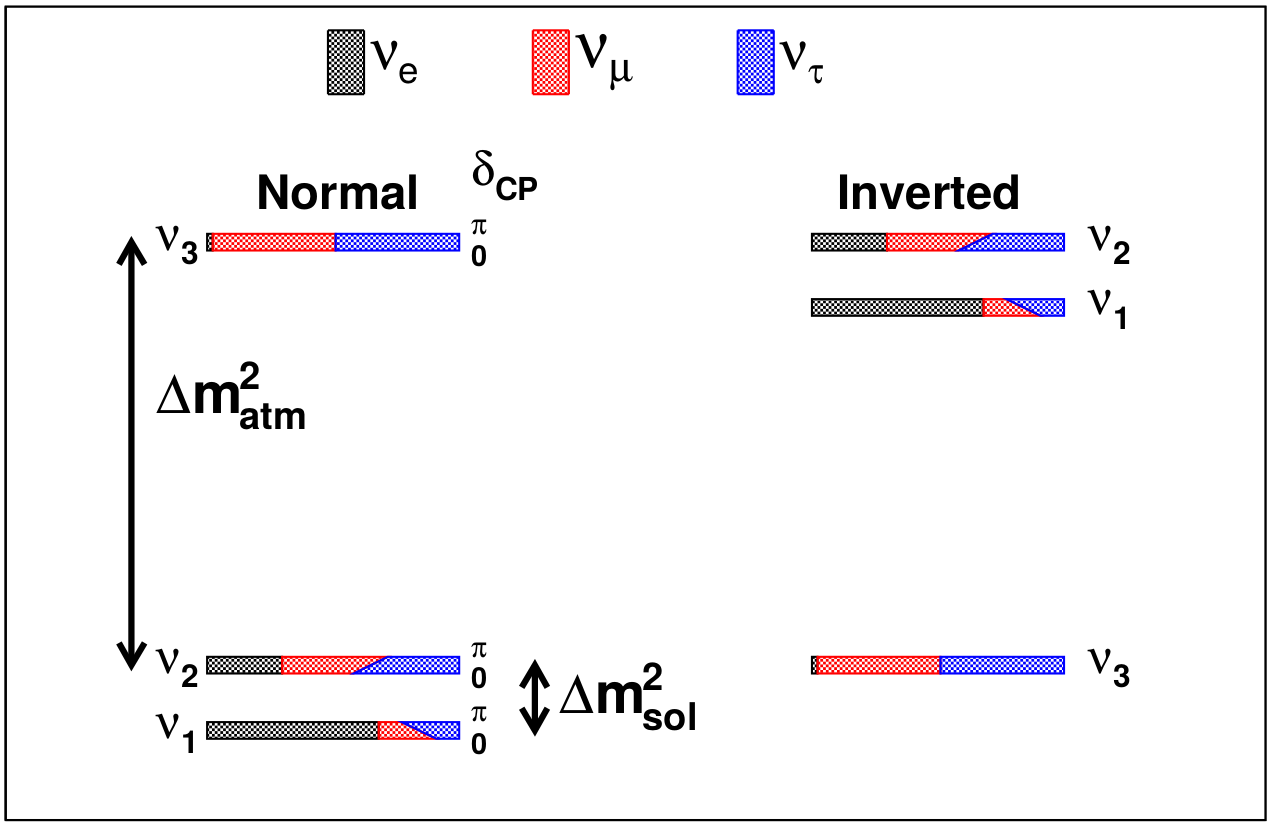
\includegraphics[width=0.5\textwidth,keepaspectratio]{mass_hierarchy.png}
		        	\caption[Les deux hiérarchies de masse possibles]{\label{fig::mass_hierarchy}Les deux hiérarchies de masse possibles et leurs composition en états de saveurs en fonction de la valeur de $\delta_{CP}$. Tiré de \cite{Qian2015}. $\Delta m^2_{sol}=\Delta m^2_{21}$ et $\Delta m^2_{atm}=\Delta m^2_{31}\simeq\Delta m^2_{32}$.}
		        \end{wrapfigure}
	            Les phénomènes observables liés aux oscillations des neutrinos font intervenir des termes de différence de masse au carré. En mesurer deux permet de calculer la troisième sans ambiguïtés. Les données expérimentales des expériences d'oscillations des neutrinos solaires et atmosphériques ont montré qu'il existe une certaine hiérarchie dans les masses des neutrinos. En effet, elles sont telles que
	            \begin{equation}\label{eq::mass_hierarchy}
	            	|\Delta m^2_{21}| <<|\Delta m^2_{31}| \simeq |\Delta m^2_{32}| 
	            \end{equation}
	            Ceci peut correspondre à quatre ordres différents pour les 3 masses $m_1$, $m_2$ et $m_3$. Parmi ces 4, deux couples sont équivalents\cite{pdg2018}, et la convention utilisée le plus souvent est celle posant $\Delta m^2_{21} > 0$. Il reste alors deux possibilités. La \autoref{fig::mass_hierarchy} montre ces deux possibilités ainsi que leur composantes respective en $\nu_e$, $\nu_{\mu}$ et $\nu_{\tau}$, pour des valeurs de $\delta_{CP}$ allant de 0 à $\pi$\cite{Qian2015}. La convention est d'appeler le cas $m_1 < m_2 < m_3$ hiérarchie normale et le cas $m_3 < m_1 < m_2$ hiérarchie inversée.
	            
	            Les premières générations d'expériences d'oscillation de neutrinos, où les effets de matières étaient absents\footnote{Sauf dans le cas des neutrinos solaires, mais la convention avait déjà posé $\Delta m^2_{21} > 0$, qui est la seule accessible par ces expériences.}, utilisaient l'approximation à deux saveurs \eqref{eq::two_flavors}, n'étant pas assez précises pour déceler des effets à trois saveurs. Le terme d'oscillation étant en $\sin^2$, il n'est pas sensible au signe de $\Delta m^2$, aussi nous ne savons toujours pas laquelle des deux hiérarchies est la bonne. Il est important de lever cette inconnue, la hiérarchie de masse est liée  un certain nombre de théories concernant la grande unification des forces fondamentales, l'origine de l'univers, ou même la production d'isotopes au sein des étoiles\cite{KH-website}.
	            
	            Une des manières de déterminer la hiérarchie de masse est d'utiliser les effets de matière. En effet, la résonance \gls{msw} dépend directement de $\Delta m^2$, comme le montre l'approximation à deux saveur \eqref{eq::MSW_condition} : si $\sin(2\theta_{13})\Delta m^2_{31} > 0$, alors on devrait pouvoir observer cette résonance en ajustant correctement l'énergie des neutrinos. Les résultats présentés dans le \autoref{tab::pmns_values} montre que $\sin(2\theta_{13}) > 0$, et donc une observation de cette résonance avec des neutrinos montrerait que la hiérarchie est normale. À l'inverse, une suppression due aux effets de matière montrerait que la hiérarchie est inversée (inversement si l'expérience est faite avec des antineutrinos). Ceci peut être fait avec des antineutrinos électroniques de réacteur, comme dans la future expérience JUNO\cite{Yang2015}, où l'on mesure la probabilité de survie de ces derniers, ou avec des (anti)neutrinos muoniques de faisceau, où l'on s'intéresse à la probabilité d'oscillation en (anti)neutrinos électroniques. Dans les deux cas, la ligne de base doit être assez importante pour donner lieu à des effets de matière conséquents.
	            
	            Dans le cadre de l'expérience \gls{dune}, la probabilité \eqref{eq::proba_matter_3flavors} et son analogue avec des antineutrinos seront mesurées et comparées à la prédiction. Les résultats attendus ainsi que les sensibilités sont présentés en \autoref{sec::dune_pheno}. 
	            
	        \subsubsection{La violation de CP et l'asymétrie matière / anti-matière}\label{sec::CP_violation}
	            La matrice \gls{pmns} a la même structure et les même propriétés que la matrice CKM qui décrit le mélange de saveur des quarks, puisque ces deux matrices décrivent le même phénomène. Dans le formalisme de la matrice CKM, C.~Jarlskog a montré que la transition d'une saveur à l'autre peut ne pas être la même entre particule et antiparticule si une certaine grandeur, appelé invariant de Jarlskog, est non nulle\cite{Jarlskog1985}. Dans le formalisme de la matrice \gls{pmns}, cette grandeur est
	            \begin{equation}
	                J_{CP}^{PMNS}=\frac{1}{8}\sin(2\theta_{12})\sin(2\theta_{13})\sin(2\theta_{23})\cos(\theta_{13})\sin(\delta_{CP}).
	            \end{equation}
	            Cette grandeur est appelé invariant car elle ne dépend pas de la paramétrisation choisie pour la phase de violation CP. On peut noter que si un seul des angles est nul, alors $J_{CP}^{PMNS}$ est nulle et les neutrinos et antineutrinos oscillent de la même manière (en absence d'effets de matière). Mais les mesures actuelles (voir \autoref{tab::pmns_values}) montrent qu'aucun des trois angles n'est nul. Dans ce cas, seule une valeur de $0$ ou $\pi$ pour $\delta_{CP}$ conserverait la symétrie CP. Les mesures les plus récentes de T2K excluent ces valeurs a $2\sigma$\cite{Abe2018} si la hiérarchie de masse est normale, mais ne sont pas assez précises pour donner une valeur exacte de $\delta_{CP}$. Or, cette valeur joue un rôle fondamental dans la question "pourquoi y a-t-il quelque chose plutôt que rien?", comme nous l'avons mentionné en \autoref{sec::CP}.
	            
	            Un papier récent\cite{Buccella2018}  a montré que, sous certaines contraintes, une valeur de $\delta_{CP}$ comprise entre $-\numprint{0.9}\pi$ et $-\numprint{0.75}\pi$ serait suffisante pour expliquer cette asymétrie. Pour ce faire, il est nécessaire d'atteindre des précisions où les oscillations à trois saveurs sont importantes. En effet, la probabilité de transition à deux saveurs \eqref{eq::two_flavors} ne fait pas intervenir $\delta_{CP}$, contrairement à la probabilité à trois saveurs \eqref{eq::proba_oscillation}. Pour les expériences à longue ligne de base, il est en plus nécessaire d'avoir une région du signal où l'effet de violation de CP dû à $\delta_{CP}$ est séparable de l'effet due aux effets de matière. En effet,  \gls{dune} mesurera la probabilité \eqref{eq::proba_matter_3flavors} et son analogue avec des antineutrinos. Les mesures seront comparées à la prédiction, les résultats attendus ainsi que les sensibilités sont présentés en \autoref{sec::dune_pheno}.
        
        \printbibliography